\documentclass[aspectratio=169]{beamer}\usepackage[]{graphicx}\usepackage[]{xcolor}
% maxwidth is the original width if it is less than linewidth
% otherwise use linewidth (to make sure the graphics do not exceed the margin)
\makeatletter
\def\maxwidth{ %
  \ifdim\Gin@nat@width>\linewidth
    \linewidth
  \else
    \Gin@nat@width
  \fi
}
\makeatother

\definecolor{fgcolor}{rgb}{0.345, 0.345, 0.345}
\newcommand{\hlnum}[1]{\textcolor[rgb]{0.686,0.059,0.569}{#1}}%
\newcommand{\hlsng}[1]{\textcolor[rgb]{0.192,0.494,0.8}{#1}}%
\newcommand{\hlcom}[1]{\textcolor[rgb]{0.678,0.584,0.686}{\textit{#1}}}%
\newcommand{\hlopt}[1]{\textcolor[rgb]{0,0,0}{#1}}%
\newcommand{\hldef}[1]{\textcolor[rgb]{0.345,0.345,0.345}{#1}}%
\newcommand{\hlkwa}[1]{\textcolor[rgb]{0.161,0.373,0.58}{\textbf{#1}}}%
\newcommand{\hlkwb}[1]{\textcolor[rgb]{0.69,0.353,0.396}{#1}}%
\newcommand{\hlkwc}[1]{\textcolor[rgb]{0.333,0.667,0.333}{#1}}%
\newcommand{\hlkwd}[1]{\textcolor[rgb]{0.737,0.353,0.396}{\textbf{#1}}}%
\let\hlipl\hlkwb

\usepackage{framed}
\makeatletter
\newenvironment{kframe}{%
 \def\at@end@of@kframe{}%
 \ifinner\ifhmode%
  \def\at@end@of@kframe{\end{minipage}}%
  \begin{minipage}{\columnwidth}%
 \fi\fi%
 \def\FrameCommand##1{\hskip\@totalleftmargin \hskip-\fboxsep
 \colorbox{shadecolor}{##1}\hskip-\fboxsep
     % There is no \\@totalrightmargin, so:
     \hskip-\linewidth \hskip-\@totalleftmargin \hskip\columnwidth}%
 \MakeFramed {\advance\hsize-\width
   \@totalleftmargin\z@ \linewidth\hsize
   \@setminipage}}%
 {\par\unskip\endMakeFramed%
 \at@end@of@kframe}
\makeatother

\definecolor{shadecolor}{rgb}{.97, .97, .97}
\definecolor{messagecolor}{rgb}{0, 0, 0}
\definecolor{warningcolor}{rgb}{1, 0, 1}
\definecolor{errorcolor}{rgb}{1, 0, 0}
\newenvironment{knitrout}{}{} % an empty environment to be redefined in TeX

\usepackage{alltt}

% Set lecture number for later use


% Part common to all the lectures
\subtitle{MATH 8xyz -- Lecture 06}
\author{\texorpdfstring{Julien Arino\newline Department of Mathematics @ University of Manitoba \newline Maud Menten Institute @ PIMS\newline\url{julien.arino@umanitoba.ca}}{Julien Arino}}
\date{Winter 20XX}

% Title of the lecture
\title{Sojourn time in compartments}



\usetheme{default}
% Slide setup, colour independent

\usepackage{amsmath,amssymb,amsthm}
\usepackage[utf8]{inputenc}
\usepackage{colortbl}
\usepackage{bm}
\usepackage{xcolor}
\usepackage{dsfont}
\usepackage{setspace}
% To use \ding{234} and the like
\usepackage{pifont}
% To cross reference between slide files
\usepackage{zref-xr,zref-user}
% Use something like
% \zexternaldocument{fileI}
% in the tex files. And cite using \zref instead of \ref
\usepackage{booktabs}
\usepackage{marvosym}
\usepackage{cancel}
%\usepackage{transparent}
% Make doi clickable in the bibliography?
\usepackage{doi}

\usepackage[T1]{fontenc}

\usepackage{longtable}

% For heavier titles
\usepackage{helvet} % Enables Helvetica font family


% Fields and the like
\def\IC{\mathbb{C}}
\def\IE{\mathbb{E}}
\def\IF{\mathbb{F}}
\def\II{\mathbb{I}}
\def\IJ{\mathbb{J}}
\def\IK{\mathbb{K}}
\def\IM{\mathbb{M}}
\def\IN{\mathbb{N}}
\def\IP{\mathbb{P}}
\def\IR{\mathbb{R}}
\newcommand{\IRplus}{\mathbb{R}_{\ge 0}}
\def\IZ{\mathbb{Z}}
\def\11{\mathds{1}}


% Bold lowercase
\def\ba{\bm{a}}
\def\bb{\bm{b}}
\def\bc{\bm{c}}
\def\bd{\bm{d}}
\def\be{\bm{e}}
\def\bf{\bm{f}}
\def\bg{\bm{g}}
\def\bh{\bm{h}}
\def\bi{\bm{i}}
\def\bj{\bm{j}}
\def\bk{\bm{k}}
\def\bn{\bm{n}}
\def\bp{\bm{p}}
\def\br{\bm{r}}
\def\bs{\bm{s}}
\def\bu{\bm{u}}
\def\bv{\bm{v}}
\def\bw{\bm{w}}
\def\bx{\bm{x}}
\def\by{\bm{y}}
\def\bz{\bm{z}}
\newcommand{\vect}[1]{\bm{#1}}

% Bold capitals
\def\bB{\bm{B}}
\def\bD{\bm{D}}
\def\bE{\bm{E}}
\def\bF{\bm{F}}
\def\bG{\bm{G}}
\def\bI{\bm{I}}
\def\bL{\bm{L}}
\def\bN{\bm{N}}
\def\bP{\bm{P}}
\def\bR{\bm{R}}
\def\bS{\bm{S}}
\def\bT{\bm{T}}
\def\bX{\bm{X}}

% Bold numbers
\def\b0{\bm{0}}

% Bold greek
\bmdefine{\bmu}{\bm{\mu}}
\def\bphi{\bm{\phi}}
\def\bvarphi{\bm{\varphi}}
\def\bPi{\bm{\Pi}}
\def\bGamma{\bm{\Gamma}}

% Bold red sentence
\def\boldred#1{{\color{red}\textbf{#1}}}
\def\defword#1{{\color{orange}\textbf{#1}}}

% Caligraphic letters
\def\A{\mathcal{A}}
\def\B{\mathcal{B}}
\def\C{\mathcal{C}}
\def\D{\mathcal{D}}
\def\E{\mathcal{E}}
\def\F{\mathcal{F}}
\def\G{\mathcal{G}}
\def\H{\mathcal{H}}
\def\I{\mathcal{I}}
\def\L{\mathcal{L}}
\def\M{\mathcal{M}}
\def\N{\mathcal{N}}
\def\P{\mathcal{P}}
\def\R{\mathcal{R}}
\def\S{\mathcal{S}}
\def\T{\mathcal{T}}
\def\U{\mathcal{U}}
\def\V{\mathcal{V}}

% Adding space for prime (') where needed
\def\pprime{\,'}
% Adding space for star (\star) where needed
\def\pstar{{\,\star}}

% tt font for code
\def\code#1{{\tt #1}}

% i.e., e.g.
\def\eg{\emph{e.g.}}
\def\ie{\emph{i.e.}}


% Operators and special symbols
\def\nbOne{{\mathchoice {\rm 1\mskip-4mu l} {\rm 1\mskip-4mu l}
{\rm 1\mskip-4.5mu l} {\rm 1\mskip-5mu l}}}
\def\cov{\ensuremath{\mathsf{cov}}}
\def\Var{\ensuremath{\mathsf{Var}\ }}
\def\Im{\textrm{Im}\;}
\def\Re{\textrm{Re}\;}
\def\det{\ensuremath{\mathsf{det}}}
\def\diag{\ensuremath{\mathsf{diag}}}
\def\nullspace{\ensuremath{\mathsf{null}}}
\def\nullity{\ensuremath{\mathsf{nullity}}}
\def\rank{\ensuremath{\mathsf{rank}}}
\def\range{\ensuremath{\mathsf{range}}}
\def\sgn{\ensuremath{\mathsf{sgn}}}
\def\Span{\ensuremath{\mathsf{span}}}
\def\tr{\ensuremath{\mathsf{tr}}}
\def\imply{$\Rightarrow$}
\def\restrictTo#1#2{\left.#1\right|_{#2}}
\newcommand{\parallelsum}{\mathbin{\!/\mkern-5mu/\!}}
\def\dsum{\mathop{\displaystyle \sum }}%
\def\dind#1#2{_{\substack{#1\\ #2}}}

\newcommand{\Qmatrix}[1]{%
  \begin{pmatrix}#1\end{pmatrix}%
}

\DeclareMathOperator{\GL}{GL}
\DeclareMathOperator{\Rel}{Re}
\def\Nt#1{\left|\!\left|\!\left|#1\right|\!\right|\!\right|}
\newcommand{\tripbar}{|\! |\! |}



% The beamer bullet (in base colour)
\def\bbullet{\leavevmode\usebeamertemplate{itemize item}\ }

% Theorems and the like
\newtheorem{proposition}[theorem]{Proposition}
\newtheorem{property}[theorem]{Property}
\newtheorem{importantproperty}[theorem]{Property}
\newtheorem{importanttheorem}[theorem]{Theorem}
%\newtheorem{lemma}[theorem]{Lemma}
%\newtheorem{corollary}[theorem]{Corollary}
\newtheorem{remark}[theorem]{Remark}
\setbeamertemplate{theorems}[numbered]
%\setbeamertemplate{theorems}[ams style]

%
%\usecolortheme{orchid}
%\usecolortheme{orchid}

\def\red{\color[rgb]{1,0,0}}
\def\blue{\color[rgb]{0,0,1}}
\def\green{\color[rgb]{0,1,0}}

% Fix skipping lines after items in the bibliography
\setbeamertemplate{bibliography entry title}{}
\setbeamertemplate{bibliography entry location}{}
\setbeamertemplate{bibliography entry note}{}

% Get rid of navigation stuff
\setbeamertemplate{navigation symbols}{}

% Set footline/header line
\setbeamertemplate{footline}
{%
\quad p. \insertpagenumber \quad--\quad \insertsection\vskip2pt
}
% \setbeamertemplate{headline}
% {%
% \quad\insertsection\hfill p. \insertpagenumber\quad\mbox{}\vskip2pt
% }


\makeatletter
\newlength\beamerleftmargin
\setlength\beamerleftmargin{\Gm@lmargin}
\makeatother

% Colours for special pages
\def\extraContent{yellow!20}


%%%%%%%%%%%%%%%%%
\usepackage{tikz}
\usetikzlibrary{shapes,arrows}
\usetikzlibrary{positioning}
\usetikzlibrary{shapes.symbols,shapes.callouts,patterns}
\usetikzlibrary{calc,fit}
\usetikzlibrary{backgrounds}
\usetikzlibrary{decorations.pathmorphing,fit,petri}
\usetikzlibrary{automata}
\usetikzlibrary{fadings}
\usetikzlibrary{patterns,hobby}
\usetikzlibrary{backgrounds,fit,petri}
\usetikzlibrary{tikzmark}

\usepackage{pgfplots}
\pgfplotsset{compat=1.6}
\pgfplotsset{ticks=none}

\usetikzlibrary{decorations.markings}
\usetikzlibrary{arrows.meta}
\tikzset{>=stealth}

% For tikz
\tikzstyle{cloud} = [draw, ellipse,fill=red!20, node distance=0.87cm,
minimum height=2em]
\tikzstyle{line} = [draw, -latex']


%%% For max frame images
\newenvironment{changemargin}[2]{%
\begin{list}{}{%
\setlength{\topsep}{0pt}%
\setlength{\leftmargin}{#1}%
\setlength{\rightmargin}{#2}%
\setlength{\listparindent}{\parindent}%
\setlength{\itemindent}{\parindent}%
\setlength{\parsep}{\parskip}%
}%
\item[]}{\end{list}}


% Make one image take up the entire slide content area in beamer,.:
% centered/centred full-screen image, with title:
% This uses the whole screen except for the 1cm border around it
% all. 128x96mm
\newcommand{\titledFrameImage}[2]{
\begin{frame}{#1}
%\begin{changemargin}{-1cm}{-1cm}
\begin{center}
\includegraphics[width=108mm,height=\textheight,keepaspectratio]{#2}
\end{center}
%\end{changemargin}
\end{frame}
}

% Make one image take up the entire slide content area in beamer.:
% centered/centred full-screen image, no title:
% This uses the whole screen except for the 1cm border around it
% all. 128x96mm
\newcommand{\plainFrameImage}[1]{
\begin{frame}[plain]
%\begin{changemargin}{-1cm}{-1cm}
\begin{center}
\includegraphics[width=108mm,height=76mm,keepaspectratio]{#1}
\end{center}
%\end{changemargin}
\end{frame}
}

% Make one image take up the entire slide area, including borders, in beamer.:
% centered/centred full-screen image, no title:
% This uses the entire whole screen
\newcommand{\maxFrameImage}[1]{
\begin{frame}[plain]
\begin{changemargin}{-1cm}{-1cm}
\begin{center}
\includegraphics[width=\paperwidth,height=\paperheight,keepaspectratio]
{#1}
\end{center}
\end{changemargin}
\end{frame}
}

% This uses the entire whole screen (to include in frame)
\newcommand{\maxFrameImageNoFrame}[1]{
\begin{changemargin}{-1cm}{-1cm}
\begin{center}
\includegraphics[width=\paperwidth,height=0.99\paperheight,keepaspectratio]
{#1}
\end{center}
\end{changemargin}
}

% Make one image take up the entire slide area, including borders, in beamer.:
% centered/centred full-screen image, no title:
% This uses the entire whole screen
\newcommand{\maxFrameImageColor}[2]{
\begin{frame}[plain]
\setbeamercolor{normal text}{bg=#2!20}
\begin{changemargin}{-1cm}{-1cm}
\begin{center}
\includegraphics[width=\paperwidth,height=\paperheight,keepaspectratio]
{#1}
\end{center}
\end{changemargin}
\end{frame}
}


\usepackage{tikz}
\usetikzlibrary{patterns,hobby}
\usepackage{pgfplots}
\pgfplotsset{compat=1.6}
\pgfplotsset{ticks=none}

\usetikzlibrary{backgrounds}
\usetikzlibrary{decorations.markings}
\usetikzlibrary{arrows.meta}
\tikzset{>=stealth}

\tikzset{
  clockwise arrows/.style={
    postaction={
      decorate,
      decoration={
        markings,
        mark=between positions 0.1 and 0.9 step 40pt with {\arrow{>}},
   }}}}


% Beginning of a section
\newcommand{\newSectionSlide}[1]{
\begin{frame}[noframenumbering,plain]
  \begin{tikzpicture}[remember picture,overlay]
    \node[above right,inner sep=0pt,opacity=0.2] at (current page.south west)
    {
        \includegraphics[height=\paperheight,width=\paperwidth]{#1}
    };
  \end{tikzpicture}
  \setbeamercolor{section in toc}{fg=section_page_list_colour}
  \setbeamerfont{section in toc}{size=\Large,series=\bfseries}
  \setbeamertemplate{section in toc shaded}[default][60]
  \tableofcontents[
    currentsection,
    sectionstyle=show/shaded,
    subsectionstyle=show/hide/hide,
    subsubsectionstyle=hide/hide/hide]
\end{frame}
\addtocounter{page}{-1}
}

% Beginning of a section in which we also show subsections
\newcommand{\newSectionWithSubsSlide}[1]{
	\begin{frame}[noframenumbering,plain]
		\begin{tikzpicture}[remember picture,overlay]
			\node[above right,inner sep=0pt,opacity=0.2] at (current page.south west)
			{
				\includegraphics[height=\paperheight,width=\paperwidth]{#1}
			};
		\end{tikzpicture}
		\setbeamercolor{section in toc}{fg=section_page_list_colour}
		\setbeamerfont{section in toc}{size=\Large,series=\bfseries}
		\setbeamertemplate{section in toc shaded}[default][60]
		\tableofcontents[
		currentsection,
		sectionstyle=show/hide,
		subsectionstyle=show/show/hide,
		subsubsectionstyle=hide/hide/hide]
	\end{frame}
	\addtocounter{page}{-1}
}

% Beginning of a subsection
\newcommand{\newSubSectionSlide}[1]{
\begin{frame}[noframenumbering,plain]
  \begin{tikzpicture}[remember picture,overlay]
    \node[above right,inner sep=0pt,opacity=0.2] at (current page.south west)
    {
        \includegraphics[height=\paperheight,width=\paperwidth]{#1}
    };
  \end{tikzpicture}
  \setbeamercolor{section in toc}{fg=subsection_page_list_colour}
  \setbeamerfont{section in toc}{size=\Large,series=\bfseries}
  \setbeamertemplate{section in toc shaded}[default][60]
  \setbeamerfont{subsection in toc}{series=\bfseries}
  \setbeamertemplate{subsection in toc shaded}[default][50]
  \tableofcontents[
    currentsection,
    sectionstyle=show/hide,
    subsectionstyle=show/shaded/hide,
    subsubsectionstyle=hide/hide/hide]
\end{frame}
\addtocounter{page}{-1}
}


% Beginning of a subsubsection
\newcommand{\newSubSubSectionSlide}[1]{
\begin{frame}[noframenumbering,plain]
  \begin{tikzpicture}[remember picture,overlay]
    \node[above right,inner sep=0pt,opacity=0.2] at (current page.south west)
    {
        \includegraphics[height=\paperheight,width=\paperwidth]{#1}
    };
  \end{tikzpicture}
  \setbeamercolor{section in toc}{fg=subsub_header_section}
  \setbeamerfont{section in toc}{size=\Large,series=\bfseries}
  \setbeamertemplate{section in toc shaded}[default][60]
  \setbeamerfont{subsection in toc}{series=\bfseries}
  \setbeamertemplate{subsection in toc shaded}[default][50]
  \setbeamertemplate{subsubsection in toc shaded}[default][50]
  \tableofcontents[
    currentsection,
    sectionstyle=show/hide,
    subsectionstyle=show/hide/hide,
    subsubsectionstyle=show/shaded/hide]
\end{frame}
\addtocounter{page}{-1}
}


   %%%%%%%%%%%
% To have links to parts in the outline
\makeatletter
\AtBeginPart{%
  \addtocontents{toc}{\protect\beamer@partintoc{\the\c@part}{\beamer@partnameshort}{\the\c@page}}%
}
%% number, shortname, page.
\providecommand\beamer@partintoc[3]{%
  \ifnum\c@tocdepth=-1\relax
    % requesting onlyparts.
    \makebox[6em]{Part #1:} \textcolor{green!30!blue}{\hyperlink{#2}{#2}}
    \par
  \fi
}
\define@key{beamertoc}{onlyparts}[]{%
  \c@tocdepth=-1\relax
}
\makeatother%

\newcommand{\nameofthepart}{}
\newcommand{\nupart}[1]%
    {   \part{#1}%
        \renewcommand{\nameofthepart}{#1}%
        {
          \setbeamercolor{background canvas}{bg=orange!50}
          \begin{frame}{#1}%\partpage 
          \hypertarget{\nameofthepart}{}\tableofcontents%
          \end{frame}
        }
    }

% This command creates a title page using TikZ only
\newcommand{\tikztitlepage}[1]{%
\begin{frame}[plain,noframenumbering]
  \begin{tikzpicture}[remember picture,overlay]
    % Background image
    \node[above right,inner sep=0pt,opacity=0.1] 
      at (current page.south west) 
      {\includegraphics[width=\paperwidth,height=\paperheight]{#1}};

    % University logo
    \node[anchor=north east, inner sep=5pt, opacity=0.9] 
      at (current page.north east)
      {
\includegraphics[width=0.2\textwidth]{FIGS-slides-admin/UM-logo-horizontal-CMYK.png}};
    
    % Title
    \node[anchor=center, align=center, 
          font=\fontsize{13}{15}\bfseries\color{UMbrown}, 
          text width=0.9\textwidth] 
          at ([yshift=2cm]current page.center)
          {\inserttitle};

      % Authors
      \node[anchor=center, align=center,
        font=\fontsize{10}{12}\bfseries\color{UMbrown},
        text width=0.7\textwidth]
        at ([yshift=0.8cm]current page.center)
        {\insertauthor};

      % Affiliation
      \node[anchor=north, align=center,
        font=\fontsize{9}{11}\color{UMbrown},
        text width=0.7\textwidth]
        at ([yshift=-0.2cm]current page.center)
        {\insertaffiliation};      
    % Date
    \node[anchor=north, align=center, 
          font=\fontsize{12}{16}\bfseries\color{UMbrown},
          text width=0.7\textwidth] 
          at ([yshift=0.2cm]current page.center)
          {\insertdate};

    % Land acknowledgement
    \node[anchor=south, align=justify, 
          font=\footnotesize, text=black, 
          text width=1.1\textwidth] 
          at ([yshift=0.5cm]current page.south)
          {The University of Manitoba campuses are located on original lands of Anishinaabeg, Ininew, Anisininew, Dakota and Dene peoples, and on the National Homeland of the Red River Métis.\\
          We respect the Treaties that were made on these territories, we acknowledge the harms and mistakes of the past, and we dedicate ourselves to move forward in partnership with Indigenous communities in a spirit of Reconciliation and collaboration.};
  \end{tikzpicture}
  \addtocounter{page}{-1}
\end{frame}
}
% The title page with figure
% \newcommand{\titlepagewithfigure}[1]{%
%   \begin{frame}[noframenumbering,plain]
%     \begin{tikzpicture}[remember picture,overlay]
%       \node[above right,inner sep=0pt,opacity=0.1] at (current page.south west)
%       {
%           \includegraphics[height=\paperheight,width=\paperwidth]{#1}
%       };
%       \node[anchor=north east,
%       inner sep=5pt,
%       opacity=0.9] at (current page.north east)
%       {
%           
\includegraphics[width=0.2\textwidth]{FIGS-slides-admin/UM-logo-horizontal-CMYK.png}
%       };
%       \node[anchor=south, 
%       align=justify, 
%       text=black, 
%       text width=1.1\textwidth,
%       font=\footnotesize]  (land_acknowledgement)
%       at (current page.south) 
%       {The University of Manitoba campuses are located on original lands of Anishinaabeg, Ininew, Anisininew, Dakota and Dene peoples, and on the National Homeland of the Red River Métis.
%       We respect the Treaties that were made on these territories, we acknowledge the harms and mistakes of the past, and we dedicate ourselves to move forward in partnership with Indigenous communities in a spirit of Reconciliation and collaboration.};  
%       % \node[align=center, anchor=south,
%       % above=0.5cm of land_acknowledgement,
%       % text=black,
%       % font=\bfseries] {\insertdate};
%   \end{tikzpicture}
%   \setbeamercolor{title}{fg=title_page_title_colour}
%   \setbeamerfont{title}{size=\Large,series=\bfseries}
%   \setbeamercolor{author}{fg=title_page_author_colour}
%   \setbeamerfont{author}{size=\large,series=\bfseries}
%   \setbeamercolor{institute}{fg=title_page_institute_colour}
%   \setbeamerfont{institute}{size=\large,series=\bfseries}
%   \setbeamercolor{date}{fg=title_page_date_colour}
%   \setbeamerfont{date}{series=\bfseries}
% 	\titlepage
% \end{frame}
% \addtocounter{page}{-1}
% }

\newcommand{\titlepagewithfigure}[1]{%
  \begin{frame}[noframenumbering,plain]
    \begin{tikzpicture}[remember picture,overlay]
      \node[above right,inner sep=0pt,opacity=0.1] at (current page.south west)
      {
          \includegraphics[height=\paperheight,width=\paperwidth]{#1}
      };
      \node[anchor=north east,
      inner sep=5pt,
      opacity=0.9] at (current page.north east)
      {
          
\includegraphics[width=0.2\textwidth]{FIGS-slides-admin/UM-logo-horizontal-CMYK.png}
      };
      \node[anchor=south, 
      align=justify, 
      text=black, 
      text width=1.1\textwidth,
      font=\footnotesize]  (land_acknowledgement)
      at (current page.south) 
      {The University of Manitoba campuses are located on original lands of Anishinaabeg, Ininew, Anisininew, Dakota and Dene peoples, and on the National Homeland of the Red River Métis.
      We respect the Treaties that were made on these territories, we acknowledge the harms and mistakes of the past, and we dedicate ourselves to move forward in partnership with Indigenous communities in a spirit of Reconciliation and collaboration.};  
      % \node[align=center, anchor=south,
      % above=0.5cm of land_acknowledgement,
      % text=black,
      % font=\bfseries] {\insertdate};
  \end{tikzpicture}
  \setbeamercolor{title}{fg=title_page_title_colour}
  \setbeamerfont{title}{size=\Large,series=\bfseries,family=\usefont{T1}{phv}{b}{n}}
  \setbeamercolor{author}{fg=title_page_author_colour}
  \setbeamerfont{author}{size=\large,series=\bfseries,family=\usefont{T1}{phv}{b}{n}}
  \setbeamercolor{institute}{fg=title_page_institute_colour}
  \setbeamerfont{institute}{size=\large,series=\bfseries,family=\usefont{T1}{phv}{b}{n}}
  \setbeamercolor{date}{fg=title_page_date_colour}
  \setbeamerfont{date}{series=\bfseries,family=\usefont{T1}{phv}{b}{n}}
	\titlepage
\end{frame}
\addtocounter{page}{-1}
}
% The outline page, with figure
% \newcommand{\outlinepage}[1]{%
% \begin{frame}[noframenumbering,plain]
%   \begin{tikzpicture}[remember picture,overlay]
%     \node[above right,inner sep=0pt,opacity=0.2] at (current page.south west)
%     {
%         \includegraphics[height=\paperheight,width=\paperwidth]{#1}
%     };
%   \end{tikzpicture}
%   \setbeamercolor{section in toc}{fg=outline_page_list_colour}
%   \setbeamerfont{section in toc}{size=\Large,series=\bfseries,family=\sffamily}
%   \frametitle{\textcolor{outline_page_title_colour}{\LARGE\bfseries Outline}}
%   \tableofcontents[hideallsubsections]
% \end{frame}
% \addtocounter{page}{-1}
% }
% The outline page, with figure
\newcommand{\outlinepage}[1]{%
\begin{frame}[noframenumbering,plain]
  \begin{tikzpicture}[remember picture,overlay]
    \node[above right,inner sep=0pt,opacity=0.2] at (current page.south west)
    {
        \includegraphics[height=\paperheight,width=\paperwidth]{#1}
    };
  \end{tikzpicture}
  \setbeamercolor{section in toc}{fg=outline_page_list_colour}
  % Use Helvetica Bold only for the outline slide TOC
  \setbeamerfont{section in toc}{size=\Large,family=\usefont{T1}{phv}{b}{n}}
  % Use Helvetica Bold for the outline title
  \frametitle{\textcolor{outline_page_title_colour}{\usefont{T1}{phv}{b}{n}\LARGE Outline}}
  \tableofcontents[hideallsubsections]
\end{frame}
\addtocounter{page}{-1}
}


%\let\oldsection\section
%\renewcommand{\section}[2]{\oldsection[#1]\newSectionSlide[#2]}





\usecolortheme{orchid}
%% Listings
\usepackage{listings}
\definecolor{mygreen}{rgb}{0,0.6,0}
\definecolor{mygray}{rgb}{0.5,0.5,0.5}
\definecolor{mymauve}{rgb}{0.58,0,0.82}
\definecolor{mygold}{rgb}{1,0.843,0}
\definecolor{myblue}{rgb}{0.537,0.812,0.941}

\definecolor{mygold2}{RGB}{120,105,22}
\definecolor{mygrey2}{RGB}{50,50,50}

\definecolor{lgreen}{rgb}{0.6,0.9,.6}
\definecolor{lred}{rgb}{1,0.5,.5}

\lstloadlanguages{R}
\lstset{ %
  language=R,
  backgroundcolor=\color{black!05},   % choose the background color
  basicstyle=\footnotesize\ttfamily,        % size of fonts used for the code
  breaklines=true,                 % automatic line breaking only at whitespace
  captionpos=b,                    % sets the caption-position to bottom
  commentstyle=\color{mygreen},    % comment style
  escapeinside={\%*}{*)},          % if you want to add LaTeX within your code
  keywordstyle=\color{red},       % keyword style
  stringstyle=\color{mygold},     % string literal style
  keepspaces=true,
  columns=fullflexible,
  tabsize=4,
}
% Could also do (in lstset)
% basicstyle==\fontfamily{pcr}\footnotesize
\lstdefinelanguage{Renhanced}%
  {keywords={abbreviate,abline,abs,acos,acosh,action,add1,add,%
      aggregate,alias,Alias,alist,all,anova,any,aov,aperm,append,apply,%
      approx,approxfun,apropos,Arg,args,array,arrows,as,asin,asinh,%
      atan,atan2,atanh,attach,attr,attributes,autoload,autoloader,ave,%
      axis,backsolve,barplot,basename,besselI,besselJ,besselK,besselY,%
      beta,binomial,body,box,boxplot,break,browser,bug,builtins,bxp,by,%
      c,C,call,Call,case,cat,category,cbind,ceiling,character,char,%
      charmatch,check,chol,chol2inv,choose,chull,class,close,cm,codes,%
      coef,coefficients,co,col,colnames,colors,colours,commandArgs,%
      comment,complete,complex,conflicts,Conj,contents,contour,%
      contrasts,contr,control,helmert,contrib,convolve,cooks,coords,%
      distance,coplot,cor,cos,cosh,count,fields,cov,covratio,wt,CRAN,%
      create,crossprod,cummax,cummin,cumprod,cumsum,curve,cut,cycle,D,%
      data,dataentry,date,dbeta,dbinom,dcauchy,dchisq,de,debug,%
      debugger,Defunct,default,delay,delete,deltat,demo,de,density,%
      deparse,dependencies,Deprecated,deriv,description,detach,%
      dev2bitmap,dev,cur,deviance,off,prev,,dexp,df,dfbetas,dffits,%
      dgamma,dgeom,dget,dhyper,diag,diff,digamma,dim,dimnames,dir,%
      dirname,dlnorm,dlogis,dnbinom,dnchisq,dnorm,do,dotplot,double,%
      download,dpois,dput,drop,drop1,dsignrank,dt,dummy,dump,dunif,%
      duplicated,dweibull,dwilcox,dyn,edit,eff,effects,eigen,else,%
      emacs,end,environment,env,erase,eval,equal,evalq,example,exists,%
      exit,exp,expand,expression,External,extract,extractAIC,factor,%
      fail,family,fft,file,filled,find,fitted,fivenum,fix,floor,for,%
      For,formals,format,formatC,formula,Fortran,forwardsolve,frame,%
      frequency,ftable,ftable2table,function,gamma,Gamma,gammaCody,%
      gaussian,gc,gcinfo,gctorture,get,getenv,geterrmessage,getOption,%
      getwd,gl,glm,globalenv,gnome,GNOME,graphics,gray,grep,grey,grid,%
      gsub,hasTsp,hat,heat,help,hist,home,hsv,httpclient,I,identify,if,%
      ifelse,Im,image,\%in\%,index,influence,measures,inherits,install,%
      installed,integer,interaction,interactive,Internal,intersect,%
      inverse,invisible,IQR,is,jitter,kappa,kronecker,labels,lapply,%
      layout,lbeta,lchoose,lcm,legend,length,levels,lgamma,library,%
      licence,license,lines,list,lm,load,local,locator,log,log10,log1p,%
      log2,logical,loglin,lower,lowess,ls,lsfit,lsf,ls,machine,Machine,%
      mad,mahalanobis,make,link,margin,match,Math,matlines,mat,matplot,%
      matpoints,matrix,max,mean,median,memory,menu,merge,methods,min,%
      missing,Mod,mode,model,response,mosaicplot,mtext,mvfft,na,nan,%
      names,omit,nargs,nchar,ncol,NCOL,new,next,NextMethod,nextn,%
      nlevels,nlm,noquote,NotYetImplemented,NotYetUsed,nrow,NROW,null,%
      numeric,\%o\%,objects,offset,old,on,Ops,optim,optimise,optimize,%
      options,or,order,ordered,outer,package,packages,page,pairlist,%
      pairs,palette,panel,par,parent,parse,paste,path,pbeta,pbinom,%
      pcauchy,pchisq,pentagamma,persp,pexp,pf,pgamma,pgeom,phyper,pico,%
      pictex,piechart,Platform,plnorm,plogis,plot,pmatch,pmax,pmin,%
      pnbinom,pnchisq,pnorm,points,poisson,poly,polygon,polyroot,pos,%
      postscript,power,ppoints,ppois,predict,preplot,pretty,Primitive,%
      print,prmatrix,proc,prod,profile,proj,prompt,prop,provide,%
      psignrank,ps,pt,ptukey,punif,pweibull,pwilcox,q,qbeta,qbinom,%
      qcauchy,qchisq,qexp,qf,qgamma,qgeom,qhyper,qlnorm,qlogis,qnbinom,%
      qnchisq,qnorm,qpois,qqline,qqnorm,qqplot,qr,Q,qty,qy,qsignrank,%
      qt,qtukey,quantile,quasi,quit,qunif,quote,qweibull,qwilcox,%
      rainbow,range,rank,rbeta,rbind,rbinom,rcauchy,rchisq,Re,read,csv,%
      csv2,fwf,readline,socket,real,Recall,rect,reformulate,regexpr,%
      relevel,remove,rep,repeat,replace,replications,report,require,%
      resid,residuals,restart,return,rev,rexp,rf,rgamma,rgb,rgeom,R,%
      rhyper,rle,rlnorm,rlogis,rm,rnbinom,RNGkind,rnorm,round,row,%
      rownames,rowsum,rpois,rsignrank,rstandard,rstudent,rt,rug,runif,%
      rweibull,rwilcox,sample,sapply,save,scale,scan,scan,screen,sd,se,%
      search,searchpaths,segments,seq,sequence,setdiff,setequal,set,%
      setwd,show,sign,signif,sin,single,sinh,sink,solve,sort,source,%
      spline,splinefun,split,sqrt,stars,start,stat,stem,step,stop,%
      storage,strstrheight,stripplot,strsplit,structure,strwidth,sub,%
      subset,substitute,substr,substring,sum,summary,sunflowerplot,svd,%
      sweep,switch,symbol,symbols,symnum,sys,status,system,t,table,%
      tabulate,tan,tanh,tapply,tempfile,terms,terrain,tetragamma,text,%
      time,title,topo,trace,traceback,transform,tri,trigamma,trunc,try,%
      ts,tsp,typeof,unclass,undebug,undoc,union,unique,uniroot,unix,%
      unlink,unlist,unname,untrace,update,upper,url,UseMethod,var,%
      variable,vector,Version,vi,warning,warnings,weighted,weights,%
      which,while,window,write,\%x\%,x11,X11,xedit,xemacs,xinch,xor,%
      xpdrows,xy,xyinch,yinch,zapsmall,zip},%
   otherkeywords={!,!=,~,$,*,\%,\&,\%/\%,\%*\%,\%\%,<-,<<-,_,/},%
   alsoother={._$},%
   sensitive,%
   morecomment=[l]\#,%
   morestring=[d]",%
   morestring=[d]'% 2001 Robert Denham
  }%

%%%%%%% 
%% Definitions in yellow boxes
\usepackage{etoolbox}
\setbeamercolor{block title}{use=structure,fg=structure.fg,bg=structure.fg!40!bg}
\setbeamercolor{block body}{parent=normal text,use=block title,bg=block title.bg!20!bg}

\BeforeBeginEnvironment{definition}{%
	\setbeamercolor{block title}{fg=black,bg=yellow!20!white}
	\setbeamercolor{block body}{fg=black, bg=yellow!05!white}
}
\AfterEndEnvironment{definition}{
	\setbeamercolor{block title}{use=structure,fg=structure.fg,bg=structure.fg!20!bg}
	\setbeamercolor{block body}{parent=normal text,use=block title,bg=block title.bg!50!bg, fg=black}
}
\BeforeBeginEnvironment{importanttheorem}{%
	\setbeamercolor{block title}{fg=black,bg=red!20!white}
	\setbeamercolor{block body}{fg=black, bg=red!05!white}
}
\AfterEndEnvironment{importanttheorem}{
	\setbeamercolor{block title}{use=structure,fg=structure.fg,bg=structure.fg!20!bg}
	\setbeamercolor{block body}{parent=normal text,use=block title,bg=block title.bg!50!bg, fg=black}
}
\BeforeBeginEnvironment{importantproperty}{%
	\setbeamercolor{block title}{fg=black,bg=red!50!white}
	\setbeamercolor{block body}{fg=black, bg=red!30!white}
}
\AfterEndEnvironment{importantproperty}{
	\setbeamercolor{block title}{use=structure,fg=structure.fg,bg=structure.fg!20!bg}
	\setbeamercolor{block body}{parent=normal text,use=block title,bg=block title.bg!50!bg, fg=black}
}

% Colour for the outline page
\definecolor{outline_colour}{RGB}{230,165,83}
%% Colours for sections, subsections aand subsubsections
\definecolor{section_colour}{RGB}{27,46,28}
\definecolor{subsection_colour}{RGB}{52,128,56}
\definecolor{subsubsection_colour}{RGB}{150,224,154}
\definecolor{subsub_header_section}{RGB}{196,44,27}
%\definecolor{mygold}{rgb}{1,0.843,0}
% Beginning of a section
% \AtBeginSection[]{
% 	{
% 	  \setbeamercolor{section in toc}{fg=mygold}
% 		\setbeamercolor{background canvas}{bg=section_colour}
% 		\begin{frame}[noframenumbering,plain]
% 			\framesubtitle{\nameofthepart Chapter \insertromanpartnumber \ -- \iteminsert{\insertpart}}
% 			\tableofcontents[
% 				currentsection,
% 				sectionstyle=show/shaded,
% 				subsectionstyle=show/hide/hide,
% 				subsubsectionstyle=hide/hide/hide]
% 		\end{frame}
% 	\addtocounter{page}{-1}
% 	%\addtocounter{framenumber}{-1} 
% 	}
% }


% % Beginning of a section
% \AtBeginSubsection[]{
% 	{
% 	  \setbeamercolor{section in toc}{fg=mygold}
% 		\setbeamercolor{background canvas}{bg=subsection_colour}
% 		\begin{frame}[noframenumbering,plain]
% 				\framesubtitle{\nameofthepart Chapter \insertromanpartnumber \ -- \iteminsert{\insertpart}}
% 				\tableofcontents[
% 					currentsection,
% 					sectionstyle=show/hide,
% 					currentsubsection,
% 					subsectionstyle=show/shaded/hide,
% 					subsubsectionstyle=show/hide/hide]
% 			\end{frame}
% 		\addtocounter{page}{-1}
% 	}
% }

% \newcommand{\newSubSectionSlide}[1]{
% \begin{frame}[noframenumbering,plain]
%   \begin{tikzpicture}[remember picture,overlay]
%     \node[above right,inner sep=0pt,opacity=0.2] at (current page.south west)
%     {
%         \includegraphics[height=\paperheight,width=\paperwidth]{#1}
%     };
%   \end{tikzpicture}
%   \setbeamercolor{section in toc}{fg=subsub_header_section}
%   \setbeamerfont{section in toc}{size=\Large,series=\bfseries}
%   \setbeamertemplate{section in toc shaded}[default][60]
%   \setbeamertemplate{subsection in toc shaded}[default][60]
%   %\setbeamercolor{background canvas}{bg=section_colour}
%   \tableofcontents[
%     currentsection,
%     sectionstyle=show/hide,
%     currentsubsection,
%     subsectionstyle=show/shaded/hide,
%     subsubsectionstyle=show/hide/hide]
% \end{frame}
% \addtocounter{page}{-1}
% }


% % Beginning of a section
% \AtBeginSubsubsection[]{
% 	{
% 	  \setbeamercolor{section in toc}{fg=subsub_header_section}
% 	  \setbeamercolor{subsubsection in toc}{fg=mygold2}
% 	  \setbeamercolor{subsubsection in toc shaded}{fg=mygrey2}
% 		\setbeamercolor{background canvas}{bg=subsubsection_colour}
% 		\begin{frame}[noframenumbering,plain]
% 				\framesubtitle{\nameofthepart Chapter \insertromanpartnumber \ -- \iteminsert{\insertpart}}
% 				\tableofcontents[
% 					currentsection,
% 					sectionstyle=show/hide,
% 					currentsubsection,
% 					subsectionstyle=show/hide/shaded
% 					currentsubsubsection]%,
% 					%subsubsectionstyle=hide/hide/shaded]
% 					%currentsubsubsection]
% 			\end{frame}
% 		\addtocounter{page}{-1}
% 	}
% }


\IfFileExists{upquote.sty}{\usepackage{upquote}}{}
\begin{document}

%%%%%%%%%%%%%%%%%%%%%%%%%%%%%%%%%
%%%%%%%%%%%%%%%%%%%%%%%%%%%%%%%%%
%% TITLE AND OUTLINE
%%%%%%%%%%%%%%%%%%%%%%%%%%%%%%%%%
%%%%%%%%%%%%%%%%%%%%%%%%%%%%%%%%%
\titlepagewithfigure{FIGS-slides-admin/Gemini_Generated_Image_uckjmbuckjmbuckj.jpeg}
\outlinepage{FIGS-slides-admin/Gemini_Generated_Image_sq8p8jsq8p8jsq8p.jpeg}


%%%%%%%%%%%%%%%%%%%
%%%%%%%%%%%%%%%%%%%
%%%%%%%%%%%%%%%%%%%
%%%%%%%%%%%%%%%%%%%
\section{Distributions of times to events}
% The section page
\newSectionSlide{FIGS-slides-admin/Gemini_Generated_Image_fu32wbfu32wbfu32.jpeg}

\begin{frame}
See some of the work of \href{https://scholar.google.ca/citations?user=o7R6ZHMAAAAJ}{Horst Thieme} on the subject
\vfill
If one considers time of sojourn in compartments from a more detailed perspective, one obtains integro-differential models
\vfill
We use here continuous random variables. See chapters 12 and 13 in \cite{thieme2018mathematics} (\href{https://press.princeton.edu/books/paperback/9780691092911/mathematics-in-population-biology}{link}) for arbitrary distributions
\end{frame}


\begin{frame}\frametitle{Time to events}
Suppose that a system can be in two states $A$ and $B$
\vfill
\begin{itemize}
\item At time $t=0$, the system is in state $A$
\vfill
\item An event happens at some time $t=\tau$, which triggers the switch from
state $A$ to state $B$
\end{itemize}
\vfill
Let $T$ be the random variable ``time spent in state $A$ before switching into state $B$''
\end{frame}

\begin{frame}
The states can be anything:
\begin{itemize}
\item $A$: working, $B$: broken
\item $A$: infected, $B$: recovered
\item $A$: alive, $B$: dead
\item $\ldots$
\end{itemize}
\vfill
We take a collection of objects or individuals that are in state $A$ and want
some law for the \defword{distribution} of the times spent in $A$, i.e., a law for $T$
\vfill
For example, we make light bulbs and would like to tell our customers that on average, our light bulbs last 200 years...
\vfill
We conduct an \defword{infinite} number of experiments, and observe the time that it takes, in every experiment, to switch from $A$ to $B$
\end{frame}

\begin{frame}
\begin{center}
  \begin{tikzpicture}[auto, %node distance = 2cm, auto,
  scale=0.8, every node/.style={transform shape},
  cloud/.style={minimum width={width("XN-1")+2pt},
  draw, ellipse,fill=blue!20}]
  \node [cloud] (S0_1) at (0,0) {$A$};
  \node [cloud] (S1_1) at (2,0) {$B$};
  \node [cloud] (S0_2) at (0,-1) {$A$};
  \node [cloud] (S1_2) at (2.5,-1) {$B$};
  \node [cloud] (S0_3) at (0,-2) {$A$};
  \node [cloud] (S1_3) at (3.5,-2) {$B$};
  \node [cloud] (S0_4) at (0,-3) {$A$};
  \node [cloud] (S1_4) at (1.5,-3) {$B$};
  %%
  \node [cloud] (S0_10) at (0,-5) {$A$};
  \node [cloud] (S1_10) at (5.5,-5) {$B$};
  %%
  \node [cloud] (S0_15) at (0,-7) {$A$};
  \node [cloud] (S1_15) at (5,-7) {$B$};
  %% Arrows
  \path [line, very thick] (S0_1) to (S1_1);
  \path [line, very thick] (S0_2) to (S1_2);
  \path [line, very thick] (S0_3) to (S1_3);
  \path [line, very thick] (S0_4) to (S1_4);
  \path [line, very thick] (S0_10) to (S1_10);
  \path [line, very thick] (S0_15) to (S1_15);
  %%
  \draw [-,-, dashed, thick] (S0_4) -- (S0_10);
  \draw [-,-, dashed, thick] (S0_10) to (S0_15);
  \draw [-,-, dashed, thick] (S0_15) to (0,-8);
  %% The time arrow
  \path [line, very thick] (0,-8.35) to (7,-8.35);
  \node[anchor=north, align=center,text=black] at (6,-8.5)
  {time}; 
  \node[anchor=north, align=center,text=black] at (0,-8.5)
  {$0$}; 
  \end{tikzpicture}
\end{center}
\end{frame}


\begin{frame}\frametitle{A distribution of probability is a model}
From the sequence of experiments, we deduce a model, which in this context is called a \defword{probability distribution}
\vfill
We assume that $T$ is a \defword{continuous} random variable
\end{frame}



\begin{frame}\frametitle{Probability density function (p.d.f.)}
Since $T$ is continuous, it has a continuous \defword{probability density function} $f$
\begin{minipage}{0.4\textwidth}
\begin{itemize}
\item $f\geq 0$
\item $\int_{-\infty}^{+\infty}f(s)ds=1$
\item $\IP(a\leq T\leq b)=\int_a^bf(t)dt$
\end{itemize}
\end{minipage}
\begin{minipage}{0.59\textwidth}
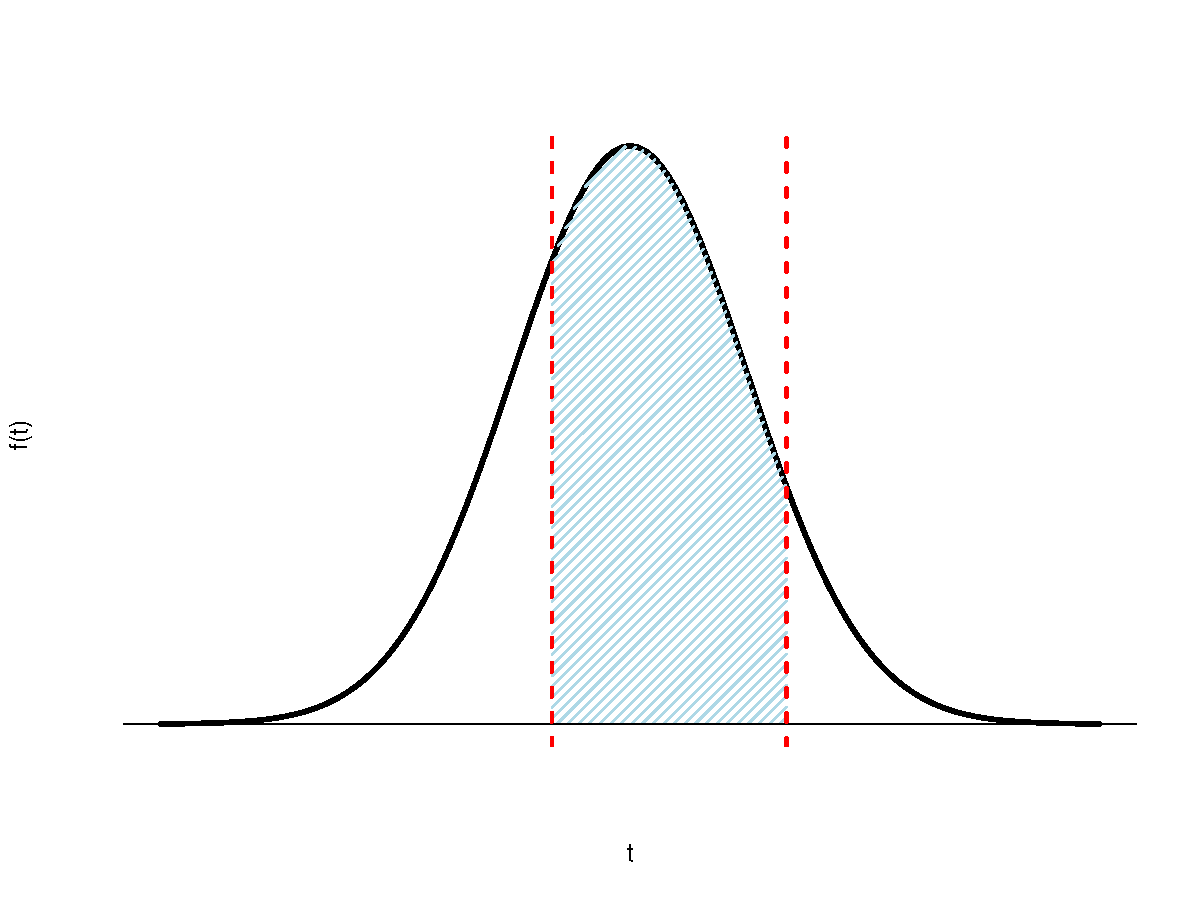
\includegraphics[width=\textwidth]{FIGS/L06-distrib_a_b-1.pdf}
\end{minipage}
\end{frame}



\begin{frame}\frametitle{Cumulative distribution function (c.d.f.)}
\begin{minipage}{0.4\textwidth}
The \defword{cumulative distribution function} is a function $F(t)$ that characterizes the distribution of $T$, and defined by
\[
F(s)=\IP(T\leq s)=\int_{-\infty}^sf(x)dx
\]
\end{minipage}
\begin{minipage}{0.59\textwidth}
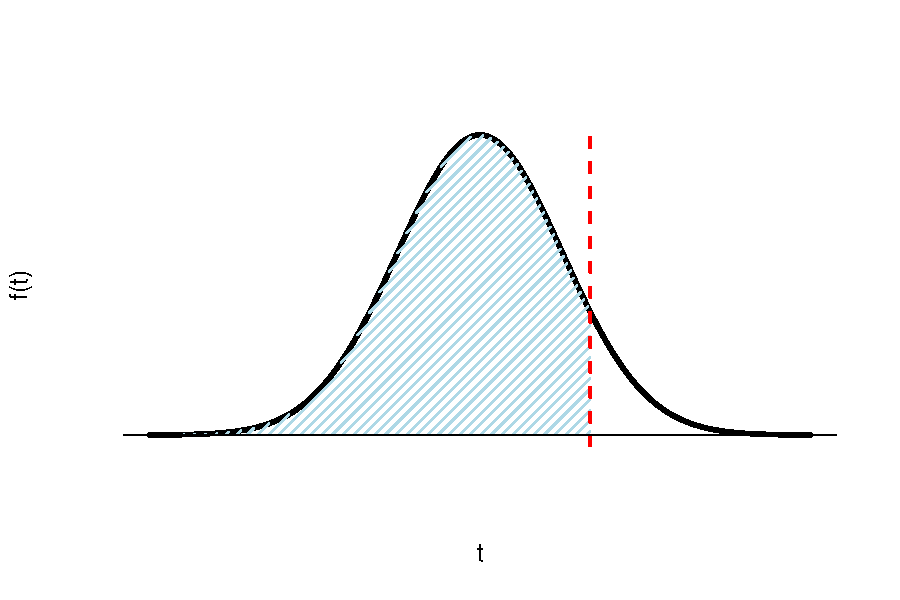
\includegraphics[width=\textwidth]{FIGS/L06-distrib_minf_b-1.pdf}
\end{minipage}
\end{frame}

\begin{frame}\frametitle{Survival function}
Another characterization of the distribution of the random variable $T$ is through the \defword{survival} (or \defword{sojourn}) function
\vfill
The survival function of state $A$ is given by 
\begin{equation}
  \S(t)=1-F(t)=\IP(T>t)
  \label{eq:survival}
\end{equation}
This gives a description of the \defword{sojourn time} of a
system in a particular state (the time spent in the state)
\vfill
$\S$ is a nonincreasing function (since $\S=1-F$
with $F$ a c.d.f.), and
$\S(0)=1$ (since $T$ is a nonnegative random variable)
\end{frame}



\maxFrameImage{FIGS/L06-pdf-cdf-surv-normal-1.pdf}

\begin{frame}
The \defword{average sojourn time} $\tau$ in state $A$ is given by
\[
\tau=E(T)=\int_0^\infty tf(t)dt
\]
Since $\lim_{t\to\infty}t\S(t)=0$, it follows that 
\[
\tau=\int_0^\infty \S(t)dt
\]
\vfill
\defword{Expected future lifetime}:
\[
\frac{1}{\S(t_0)} \int_0^{\infty} t\,f(t+t_0)\,dt 
\]
\vfill
\begin{eqnarray*}
\S(t)-\S(a)&=&\IP\left\{\textrm{survive during }
 (a,t)\textrm{ having survived until }a\right\} \\
&=& \exp\left(-\int_a^t h(u)du\right)
\end{eqnarray*}
\end{frame}

\begin{frame}\frametitle{Hazard rate}
The \defword{hazard rate} (or \defword{failure rate}) is
\begin{align*}
h(t) &= \lim_{\Delta t\to 0}\frac{\S(t)-\S(t+\Delta t)}{\Delta t} \\
& = \lim_{\Delta t\to 0} \frac{\IP(T<t+\Delta t | T\geq
t)}{\Delta t} \\
&= \frac{f(t)}{\S(t)}
\end{align*}
It gives probability of failure between $t$ and $\Delta t$, given survival to $t$.
\vfill
We have
\[
h(t)=-\frac{d}{dt}\ln\S(t)
\]
\end{frame}



\maxFrameImage{FIGS/L06-pdf-cdf-surv-hazard-normal-1.pdf}

%%%%%%%%%%%%%%%%%%%%%%%%%%%
\begin{frame}{Competing risks}
Suppose now that the system starts in state $A$ at time $t=0$ and that depending on which of the two events $\mathcal{E}_1$ or $\mathcal{E}_2$ takes place first, it switches to state $B_1$ or $B_2$, respectively
\vfill
Consider the random variables $T_A$, \emph{time spent} in state $A$ (or sojourn time in $A$), $T_{AB_1}$, \emph{time before switch to} $B_1$ and $T_{AB_2}$, \emph{time before switch to} $B_2$
\vfill
If we consider state $A$, we cannot observe the variables $T_{AB_1}$ or $T_{AB_2}$. What is observable is the sojourn time in $A$
\[
T^*_A=\min\left( T_{AB_1},T_{AB_2} \right)
\]
(where $^*$ indicates that a quantity is observable)
\end{frame}

\begin{frame}{Failure rate by type of event}
We have two (or more) types of events whose individual failure rates have to be accounted for
\begin{align*}
h_j(t) &= \lim_{\Delta t\to 0} \frac{\mathbb{P}( T<t+\Delta t, S=S_j | T\geq t)}{\Delta t} 
\end{align*}
where $\mathbb{P}(T<t+\Delta t, S=S_j | T\geq t)$ is the probability of failure due to cause $S_j$ ($j=1,2$ ici), i.e., $S$ is a discrete r.v. representing the event that is taking place
\end{frame}

\begin{frame}
By the law of total probability, since only one of the event can take place, if there are $n$ risks, then
$$
h(t) = \sum_{i=1}^n h_j(t)
$$
or, identically,
$$
\mathcal{S}(t)
=
\exp\left(
  -\int_0^t \sum\textstyle_{j=1}^n h_j(s)\ ds
\right)
$$
\end{frame}

\begin{frame}
As a consequence, suppose a process is subject to two competing exponential risks with respective distributions with parameters $\theta_1$ and $\theta_2$
\vfill
Then the mean sojourn time in the initial state before being affected by one of the two risks is
$$
\frac{1}{\theta_1+\theta_2}
$$
\end{frame}


%%%%%%%%%%%%%%%%%%%
%%%%%%%%%%%%%%%%%%%
%%%%%%%%%%%%%%%%%%%
%%%%%%%%%%%%%%%%%%%
\section{Two ``extreme'' distributions and a nicer one}
% The section page
\newSectionSlide{FIGS-slides-admin/Gemini_Generated_Image_5yvymh5yvymh5yvy.jpeg}

\begin{frame}\frametitle{The exponential distribution}
The random variable $T$ has an \defword{exponential} distribution if its
probability density function takes the form
\begin{equation}\label{eq:exp_distrib}
f(t)=\begin{cases}0&\textrm{if }t<0,\\
\theta e^{-\theta t}&\textrm{if }t\geq 0,
\end{cases}
\end{equation}
with $\theta>0$. Then the
survival function for state $A$ is of the form $\S(t)=e^{-\theta
  t}$, for $t\geq 0$, and the average sojourn time in state $A$ is
\[
\tau=\int_0^\infty e^{-\theta t}dt=\frac 1\theta
\]
\end{frame}

\begin{frame}\frametitle{Particularities of the exponential distribution}
The standard deviation of an exponential distribution is also $1/\theta$. When estimating $\theta$, it is impossible to distinguish the mean and the standard deviation
\vfill
The exponential distribution is \defword{memoryless}: its conditional probability obeys
\[
P(T > s + t\; |\; T > s) = P(T > t),\quad\forall s, t \ge 0
\]

The exponential and geometric distributions are the only memoryless probability distributions
\vfill
The exponential distribution has a constant hazard function $h(t)\equiv\theta$
\end{frame}



\maxFrameImage{FIGS/L06-pdf-cdf-surv-hazard-expon-1.pdf}

\begin{frame}\frametitle{The Dirac delta distribution}
If for some constant $\omega>0$,
\[
\S(t)=
\left\{
\begin{array}{ll}
1, & 0\leq t\leq\omega \\
0, & \omega<t
\end{array}
\right.
\]
meaning that $T$ has a Dirac delta distribution
$\delta_\omega(t)$, then the average sojourn time is
\[
\tau=\int_0^\omega dt=\omega
\]
with standard deviation $\sigma=0$
\end{frame}

\begin{frame}{The Gamma distribution}
R.v. $X$ is \defword{Gamma} distributed ($X\,\sim\Gamma(k, \theta)$) with \defword{shape parameter} $k$ and \defword{scale parameter} $\theta$ (or \defword{rate} $\beta = 1/\theta$) (all positive) if its probability density function takes the form
\begin{equation}\label{eq:gamma_distrib}
f(x;k,\theta) = \frac{x^{k-1} \mathrm{e}^{-\frac{x}{\theta}}}{\Gamma ( k)\theta ^k}
\end{equation}
where $x>0$ and $\Gamma$ is the Euler Gamma function, defined for all $z\in\mathbb{C}$ s.t. $\Re(z) > 0$ by
\[
\Gamma : z \mapsto \int_0^{+\infty}  t^{z-1}\,\mathrm{e}^{-t}\,\mathrm{d}t
\]
\end{frame}

\begin{frame}{Properties of the Gamma distribution}
Mean $k\theta$, variance $k\theta^2$
\vfill
Survival function
\[
\mathcal{S}(t)=
1-\frac{1}{\Gamma(k)}\gamma\left(
k,\frac{t}{\theta} 
\right)
=1-\frac{1}{\Gamma(k)}\gamma\left(
k,\beta t
\right)
\]
where 
\[
\gamma(a,x)=\int_0^x t^{a-1}{\rm e}^{-t}{\rm d}t
\]
is an incomplete Gamma function
\end{frame}



\maxFrameImage{FIGS/L06-pdf-cdf-surv-hazard-gamma-1.pdf}


%%%%%%%%%%%%%%%%%%%
%%%%%%%%%%%%%%%%%%%
%%%%%%%%%%%%%%%%%%%
%%%%%%%%%%%%%%%%%%%
\section{A simple cohort model with death} 
% The section page
\newSectionSlide{FIGS-slides-admin/Gemini_Generated_Image_5yvymh5yvymh5yvy.jpeg}

\begin{frame}\frametitle{A model for a cohort with one cause of death}
Consider a \defword{cohort} of individuals born at the same time, e.g., the same year
\vfill
\begin{itemize}
\item At time $t=0$, there are initially $N_0>0$ individuals
\item All causes of death are compounded together 
\item The time until death, for a given individual, is a random variable $T$, with continuous probability density distribution $f(t)$ and survival function $\S(t)$
\end{itemize}
\vfill
$N(t)$ the cohort population at time $t\geq 0$
\begin{equation}\label{eq:N_general}
N(t)=N_0\S(t)
\end{equation}
\vfill
$\S(t)$ proportion of initial population still alive at time $t$, so $N_0\S(t)$ number in the cohort still alive at time $t$
\end{frame}

\begin{frame}\frametitle{Case where $T$ is exponentially distributed}
Suppose that $T$ has an exponential distribution with mean $1/d$ (or parameter $d$), $f(t)=de^{-dt}$. Then the survival function is $\S(t)=e^{-dt}$, and \eqref{eq:N_general} takes the form
\begin{equation}\label{eq:N}
N(t)=N_0e^{-dt}
\end{equation}
\vfill
Now note that
\begin{align*}
\frac{d}{dt} N(t) &= -dN_0e^{-dt} \\
&= -dN(t)
\end{align*}
with $N(0)=N_0$.
\vfill
{\red $\Rightarrow$} The ODE $N'=-dN$ makes the assumption that the life expectancy at birth is exponentially distributed
\end{frame}



\begin{frame}
Survival function, $\S(t)=\IP(T>t)$, for an exponential distribution with mean 80 years
\begin{center}
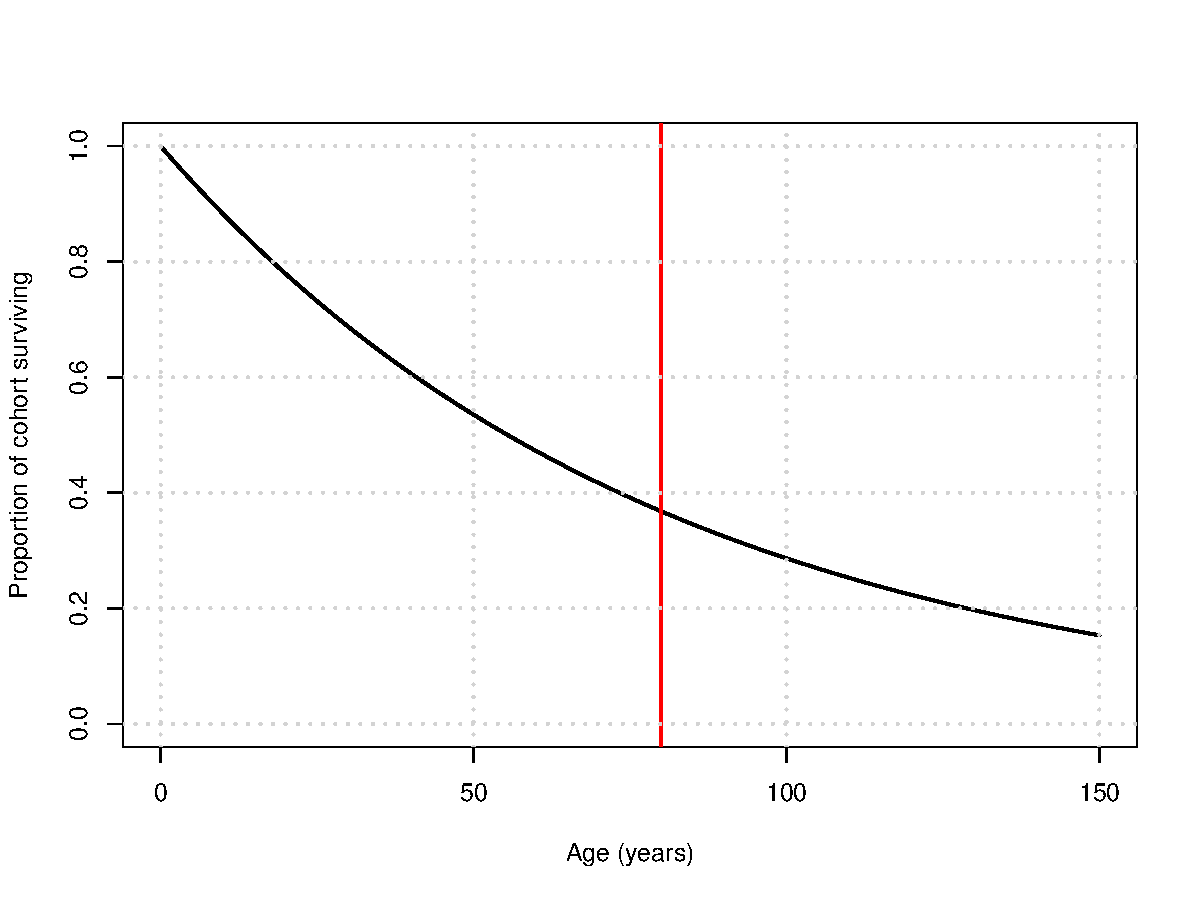
\includegraphics[width=0.8\textwidth]{FIGS/L06-prop_surviving_exp_80years-1.pdf}
\end{center}
\end{frame}


\begin{frame}\frametitle{Case where $T$ has a Dirac delta distribution}
Suppose that $T$ has a Dirac delta distribution at $t=\omega$, giving the
survival function 
\[
\S(t)=\begin{cases}
1, & 0\leq t\leq\omega \\
0, & t>\omega 
\end{cases}
\]
Then \eqref{eq:N_general} takes the form
\begin{equation}\label{eq:N2}
N(t)=\begin{cases}
N_0, & 0\leq t\leq\omega \\
0, & t>\omega
\end{cases}
\end{equation}
All individuals survive until time $\omega$, then they all die at time $\omega$
\vfill
Here, $N'=0$ everywhere except at $t=\omega$, where it is undefined
\end{frame}




\begin{frame}
Survival function, $\S(t)=\IP(T>t)$, for a Dirac distribution with mean 80 years
\begin{center}
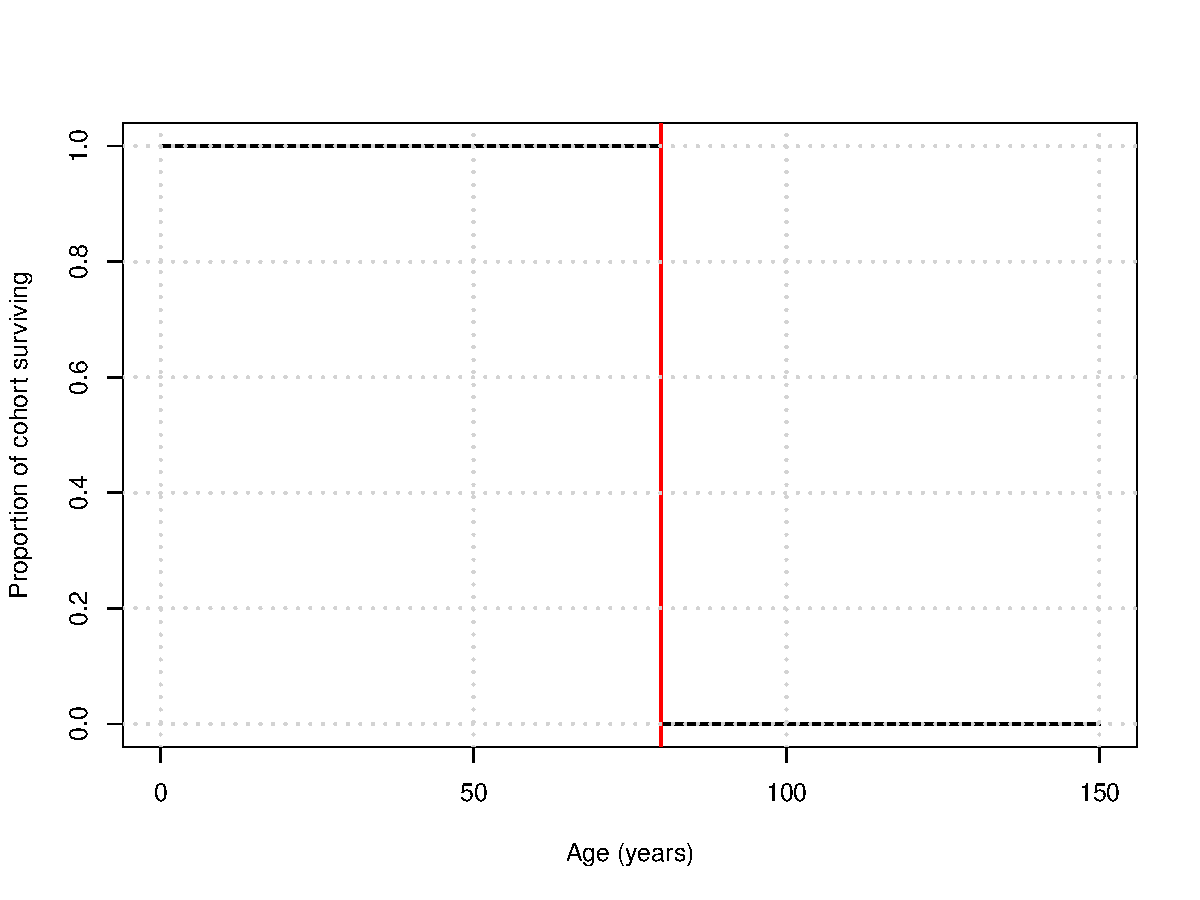
\includegraphics[width=0.8\textwidth]{FIGS/L06-prop_surviving_dirac_80years-1.pdf}
\end{center}
\end{frame}




%%%%%%%%%%%%%%%%%%%
%%%%%%%%%%%%%%%%%%%
%%%%%%%%%%%%%%%%%%%
%%%%%%%%%%%%%%%%%%%
\section{Possible fixes to the exponential distribution issue} 
% The section page
\newSectionSlide{FIGS-slides-admin/Gemini_Generated_Image_5yvymh5yvymh5yvy.jpeg}

%%%%%%%%%%%%%%%%%%%
%%%%%%%%%%%%%%%%%%%
\subsection{The issue with exponential distributions} 
% The section page
\newSubSectionSlide{FIGS-slides-admin/Gemini_Generated_Image_5yvymh5yvymh5yvy.jpeg}



\begin{frame}{Survival for the exponential distribution}
\begin{center}
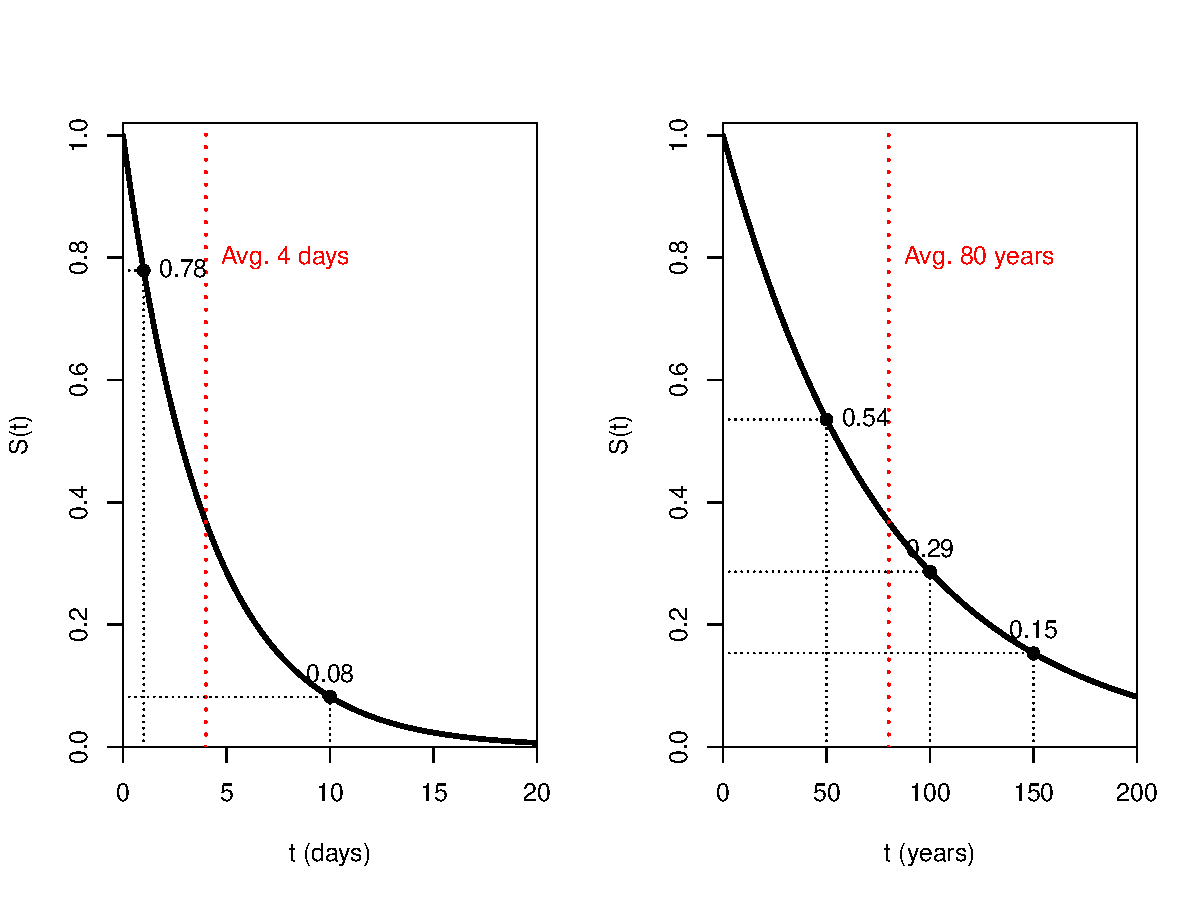
\includegraphics[width=0.75\textwidth]{FIGS/L06-prop_surviving_exp_80years_details-1.pdf}
\end{center}
\end{frame}

\begin{frame}{Issues with the exponential distribution}
\bbullet Survival drops quickly
\vfill
\bbullet Survival continues way beyond the mean
\vfill
Acceptable if what matters is the average duration of sojourn in a compartment (e.g., long term dynamics)
\vfill
More iffy if one is interested in short-term dynamics
\vfill
\bbullet Exponential distribution with parameter $\theta$ has same mean and standard deviation $1/\theta$, i.e., a single parameter controls mean and dispersion about the mean
\end{frame}

%%%%%%%%%%%%%%%%%%%
%%%%%%%%%%%%%%%%%%%
\subsection{Fix 1 -- Use info on the distribution as well}
% The section page
\newSubSectionSlide{FIGS-slides-admin/Gemini_Generated_Image_5yvymh5yvymh5yvy.jpeg}

%%%%%%%%%%%%%%%%%%%
%%%%%%%%%%%%%%%%%%%
\subsection{Fix 2 -- Use an Erlang distribution} 
% The section page
\newSubSectionSlide{FIGS-slides-admin/Gemini_Generated_Image_5yvymh5yvymh5yvy.jpeg}


\begin{frame}
    \frametitle{Side note -- What is a convolution?}
    \begin{itemize}
        \item The \emph{convolution product} is used to find the probability distribution of the \emph{sum of two independent random variables}
        \vfill
        \item If $X$ and $Y$ are two continuous random variables, and $Z = X + Y$, use the convolution to find the p.d.f. $f_Z(z)$ of $Z$
    \end{itemize}
\end{frame}

\begin{frame}
    \frametitle{The setting}
    \begin{itemize}
        \item Consider two independent continuous random variables $X$ and $Y$ with p.d.f. $f_X(x)$ and $f_Y(y)$, respectively
        \vfill
        \item Want to find the p.d.f. of their sum $Z = X + Y$
        \vfill
        \item Simply adding the p.d.f. or multiplying them does not yield the correct distribution for the sum $Z$
        \vfill
        \item Convolution accounts for all possible combinations of $X$ and $Y$ that sum to a specific value $z$
    \end{itemize}
\end{frame}

\begin{frame}
    \frametitle{Deriving the convolution formula}
    Start with the c.d.f. of $Z$:
    \begin{itemize}
        \item $F_Z(z) = \IP(Z \le z) = \IP(X + Y \le z)$
        \item Since $X$ and $Y$ are independent, their joint p.d.f. is $f_{X,Y}(x,y) = f_X(x)f_Y(y)$
        \item $\IP(X + Y \le z)$ found by integrating the joint p.d.f. over the region where $x+y \le z$
        $$ F_Z(z) = \iint_{x+y \le z} f_X(x)f_Y(y) \,dx\,dy $$
        \item Change the order of integration. For a fixed $x$, $y$ must be less than or equal to $z-x$
        $$ F_Z(z) = \int_{-\infty}^{\infty} \left( \int_{-\infty}^{z-x} f_Y(y) \,dy \right) f_X(x) \,dx $$
        \item Inner integral is c.d.f. of $Y$ evaluated at $z-x$, i.e., $F_Y(z-x)$
        $$ F_Z(z) = \int_{-\infty}^{\infty} F_Y(z-x) f_X(x) \,dx $$
    \end{itemize}
\end{frame}

\begin{frame}
    \frametitle{Deriving the convolution formula (2)}
    To obtain the PDF $f_Z(z)$, we differentiate the CDF $F_Z(z)$ with respect to $z$
    \vfill
    \begin{itemize}
        \item $f_Z(z) = \frac{d}{dz} F_Z(z) = \frac{d}{dz} \int_{-\infty}^{\infty} F_Y(z-x) f_X(x) \,dx $
        \vfill
        \item Using Leibniz integral rule (differentiating under the integral sign)
        $$ f_Z(z) = \int_{-\infty}^{\infty} \frac{\partial}{\partial z} F_Y(z-x) f_X(x) \,dx $$
        \vfill
        \item Since $\frac{d}{du} F_Y(u) = f_Y(u)$, and here $u = z-x$, we have $\frac{\partial}{\partial z} F_Y(z-x) = f_Y(z-x)$
    \end{itemize}
\end{frame}

\begin{frame}
    \frametitle{The convolution pProduct formula}
    $$ f_Z(z) = \int_{-\infty}^{\infty} f_X(x) f_Y(z-x) \,dx $$
    \vfill
    \begin{itemize}
        \item This is the \defword{convolution product} of $f_X$ and $f_Y$, often denoted as $(f_X * f_Y)(z)$
        \vfill
        \item Alternatively, by symmetry
        $$ f_Z(z) = \int_{-\infty}^{\infty} f_Y(y) f_X(z-y) \,dy $$
        \vfill
        \item \textbf{Key condition --} Valid only if $X$ and $Y$ are \emph{independent} r.v.
    \end{itemize}
\end{frame}

\begin{frame}{Exponential distributions are ``bad'' but also cool}
$X_1$ and $X_2$ 2 i.i.d. (independent and identically distributed) exponential r.v. with parametres $\theta_1$ and $\theta_2$. Then the probability density function of the r.v. $Z=X_1+X_2$ is given by the convolution
\begin{align}
 f_Z(z) &= \int_{-\infty}^\infty f_{X_1}(x_1) f_{X_2}(z - x_1)\,dx_1 \nonumber\\
   &= \int_0^z \theta_1 e^{-\theta_1 x_1} \theta_2 e^{-\theta_2(z - x_1)} \, dx_1 \nonumber\\
   &= \theta_1 \theta_2 e^{-\theta_2 z} \int_0^z e^{(\theta_2 - \theta_1)x_1}\,dx_1 \nonumber\\
   &= \begin{cases}
        \dfrac{\theta_1 \theta_2}{\theta_2-\theta_1} \left(e^{-\theta_1 z} - e^{-\theta_2 z}\right) & \text{ if } \theta_1 \neq \theta_2 \\
        \theta^2 z e^{-\theta z} & \text{ if } \theta_1 = \theta_2 =: \theta
      \end{cases}
\end{align}
\end{frame}

\begin{frame}{The tool we use}
\begin{theorem}
Let $X_i$ be independent exponentially distributed random variables with parameter $\xi$ and $Y = \sum_{i=1}^n X_i$
\vskip1cm
Then the random variable $Y\rightsquigarrow E(n,\xi)$, an Erlang distribution with \emph{shape} parameter $n$ and \emph{scale} parameter $\xi$
\end{theorem}
\vfill
(Erlang distribution: Gamma distribution with integer shape parameter)
\end{frame}

\begin{frame}{Consequences for compartmental models}
If $n$ compartments are traversed successively by individuals, with each compartment having an outflow rate of $1/\xi$ (or a mean sojourn time of $\xi$), then the time of sojourn from entry into the first compartment to exit from the last is Erlang distributed with mean $E(Y)=n\xi$ and variance $\mathsf{Var}(Y)=n\xi^2$
\vfill
\begin{center}
\def\skip{*3}
\begin{tikzpicture}[scale=0.5, 
every node/.style={transform shape},
auto,
box/.style={minimum size=1.5cm, 
draw=black, very thick},
draw, circle]
%% States (imported original variants)
\node [box, fill=gray!20] at (0\skip,8) (X) {$X$};
\node [box, fill=gray!20] at (0\skip,4) (X1) {$X_{1}$};
\node [box, fill=gray!20] at (1\skip,4) (X2) {$X_{2}$};
\node [box, fill=gray!20] at (3\skip,4) (Xk) {$X_{k}$};
\node [box, fill=gray!20] at (5\skip,4) (XNm1) {$X_{N-1}$};
\node [box, fill=gray!20] at (6\skip,4) (XN) {$X_{N}$};
% Metabox
\draw [blue,rounded corners, thick, fill=blue!40, fill opacity=0.2] (-0.5\skip,9) -- (7\skip,9) -- (7\skip, 7) -- (-0.5\skip, 7) -- cycle;
\draw [blue,rounded corners, thick, fill=blue!40, fill opacity=0.2] (-0.5\skip,5) -- (7\skip,5) -- (7\skip, 3) -- (-0.5\skip, 3) -- cycle;
%% Flows (exponential box)
\path [line, very thick] (X) to node [midway, above] (TextNode) {$\mu X$} (7\skip,8);
%% Flows (Erlang box)
\path [line, very thick] (X1) to node [midway, above] (TextNode) {$\varepsilon X_1$} (X2);
\path [line, very thick] (X2) to node [midway, above] (TextNode) {$\varepsilon X_2$} (2\skip,4);
\path [line, very thick] (4\skip,4) to node [midway, above] (TextNode) {$\varepsilon X_{N-2}$} (XNm1);
\path [line, very thick] (XNm1) to node [midway, above] (TextNode) {$\varepsilon X_{N-1}$} (XN);
\path [line, very thick] (XN) to node [midway, above] (TextNode) {$\varepsilon X_{N}$} (7\skip,4);
%% To and from centre node
\path [line, very thick, dashed] (2.25\skip,4) to node [midway, above] (TextNode) {} (Xk);
\path [line, very thick, dashed] (Xk) to node [midway, above] (TextNode) {} (3.75\skip,4);
%% Time lines
\draw [|-|, thick] (0\skip,6.5) -- (7\skip,6.5);
\draw [|-|, thick] (0\skip,2.5) -- (7\skip,2.5);
%% Labels of time lines 
\node at (6\skip,2) {Average sojourn time $N/\varepsilon$};
\node at (6\skip,6) {Average sojourn time $1/\mu$};
\end{tikzpicture}
\end{center}
\vfill
I have a \href{https://daytah-or-dahtah.ovh:3838/Erlang_shiny/}{Shiny app} for this :)
\end{frame}

%%%%%%%%%%%%%%%%%%%
%%%%%%%%%%%%%%%%%%%
\subsection{Finding the right Erlang} 
% The section page
\newSubSectionSlide{FIGS-slides-admin/Gemini_Generated_Image_5yvymh5yvymh5yvy.jpeg}

\begin{frame}{Example: EVD incubation periods}
During the 2014 Ebola Virus Disease (EVD) crisis in Western Africa, the WHO Ebola Response Team estimated incubation periods in a 2015 paper
\vfill
Table S2 in the Supplementary Information in that paper gives the best fit for the distribution of incubation periods for EVD as a Gamma distribution with mean 10.3 days and standard deviation 8.2, i.e., $n\varepsilon = 10.3$ and $\varepsilon \sqrt{n}=8.2$
\vfill
From this, $\varepsilon = 8.2^2/10.3 \simeq 6.53$ and $n = 10.3^2/8.2^2 \simeq 1.57$. However, that is a Gamma distribution
\end{frame}

\begin{frame}[fragile]{Switching to a compartmental model approach}
To use multiple compartments to better fit residence times, we need to find the closest possible Erlang distribution to this Gamma distribution
\vfill
$\implies$ compute RSS errors between data points generated from the given Gamma distribution and an Erlang
\vfill 
\begin{knitrout}
\definecolor{shadecolor}{rgb}{0.969, 0.969, 0.969}\color{fgcolor}\begin{kframe}
\begin{alltt}
\hldef{error_Gamma} \hlkwb{<-} \hlkwa{function}\hldef{(}\hlkwc{theta}\hldef{,}\hlkwc{shape}\hldef{,}\hlkwc{t}\hldef{,}\hlkwc{data}\hldef{) \{}
  \hldef{test_points} \hlkwb{<-} \hlkwd{dgamma}\hldef{(t,} \hlkwc{shape} \hldef{= shape,} \hlkwc{scale} \hldef{= theta)}
  \hldef{ls_error} \hlkwb{<-} \hlkwd{sum}\hldef{((data}\hlopt{-}\hldef{test_points)}\hlopt{^}\hlnum{2}\hldef{)}
  \hlkwd{return}\hldef{(ls_error)}
\hldef{\}}
\end{alltt}
\end{kframe}
\end{knitrout}

\end{frame}

\begin{frame}[fragile, allowframebreaks]

\begin{knitrout}
\definecolor{shadecolor}{rgb}{0.969, 0.969, 0.969}\color{fgcolor}\begin{kframe}
\begin{alltt}
\hldef{optimize_gamma} \hlkwb{<-} \hlkwa{function}\hldef{(}\hlkwc{t}\hldef{,}\hlkwc{d}\hldef{) \{}
  \hldef{max_shape} \hlkwb{<-} \hlnum{10}
  \hldef{error_vector} \hlkwb{<-} \hlkwd{mat.or.vec}\hldef{(max_shape,}\hlnum{1}\hldef{)}
  \hldef{scale_vector} \hlkwb{<-} \hlkwd{mat.or.vec}\hldef{(max_shape,}\hlnum{1}\hldef{)}
  \hlkwa{for} \hldef{(i} \hlkwa{in} \hlnum{1}\hlopt{:}\hldef{max_shape) \{}
    \hldef{result_optim} \hlkwb{<-} \hlkwd{try}\hldef{(}\hlkwd{optim}\hldef{(}\hlkwc{par} \hldef{=} \hlnum{3}\hldef{,}
                              \hlkwc{fn} \hldef{= error_Gamma,}
                              \hlkwc{lower} \hldef{=} \hlnum{0}\hldef{,}
                              \hlkwc{method} \hldef{=} \hlsng{"L-BFGS-B"}\hldef{,}
                              \hlkwc{shape} \hldef{= i,}
                              \hlkwc{t} \hldef{= t,}
                              \hlkwc{data} \hldef{= d),}
                        \hlnum{TRUE}\hldef{)}
    \hlkwa{if} \hldef{(}\hlopt{!}\hlkwd{inherits}\hldef{(result_optim,}\hlsng{"try-error"}\hldef{)) \{}
      \hldef{error_vector[i]} \hlkwb{<-} \hldef{result_optim}\hlopt{$}\hldef{value}
      \hldef{scale_vector[i]} \hlkwb{<-} \hldef{result_optim}\hlopt{$}\hldef{par}
    \hldef{\}} \hlkwa{else} \hldef{\{}
      \hldef{error_vector[i]} \hlkwb{<-} \hlnum{NaN}
      \hldef{scale_vector[i]} \hlkwb{<-} \hlnum{NaN}
    \hldef{\}}
  \hldef{\}}
  \hldef{result_optim} \hlkwb{<-} \hlkwd{data.frame}\hldef{(}\hlkwd{seq}\hldef{(}\hlnum{1}\hldef{,max_shape),}
                             \hldef{scale_vector,}
                             \hldef{error_vector)}
  \hlkwd{colnames}\hldef{(result_optim)} \hlkwb{<-} \hlkwd{c}\hldef{(}\hlsng{"shape"}\hldef{,}\hlsng{"scale"}\hldef{,}\hlsng{"error"}\hldef{)}
  \hldef{result_optim} \hlkwb{<-} \hldef{result_optim[}\hlkwd{complete.cases}\hldef{(result_optim),]}
  \hlkwd{return}\hldef{(result_optim)}
\hldef{\}}
\end{alltt}
\end{kframe}
\end{knitrout}

\end{frame}


\begin{frame}[fragile]

\begin{knitrout}
\definecolor{shadecolor}{rgb}{0.969, 0.969, 0.969}\color{fgcolor}\begin{kframe}
\begin{alltt}
\hldef{time_points} \hlkwb{<-} \hlkwd{seq}\hldef{(}\hlnum{0}\hldef{,}\hlnum{60}\hldef{)}
\hldef{data_points} \hlkwb{<-} \hlkwd{dgamma}\hldef{(time_points,} \hlkwc{shape} \hldef{=} \hlnum{1.57}\hldef{,}
                      \hlkwc{scale} \hldef{=} \hlnum{6.53}\hldef{)}
\hlcom{# Run the minimization}
\hldef{optim_fits} \hlkwb{<-} \hlkwd{optimize_gamma}\hldef{(time_points,data_points)}
\hlcom{# Which is the best Erlang to fit the data}
\hldef{idx_best} \hlkwb{<-} \hlkwd{which.min}\hldef{(optim_fits}\hlopt{$}\hldef{error)}
\end{alltt}
\end{kframe}
\end{knitrout}

\end{frame}



\begin{frame}
We find the best fit below, which is obtained using 2 compartments
\begin{center}
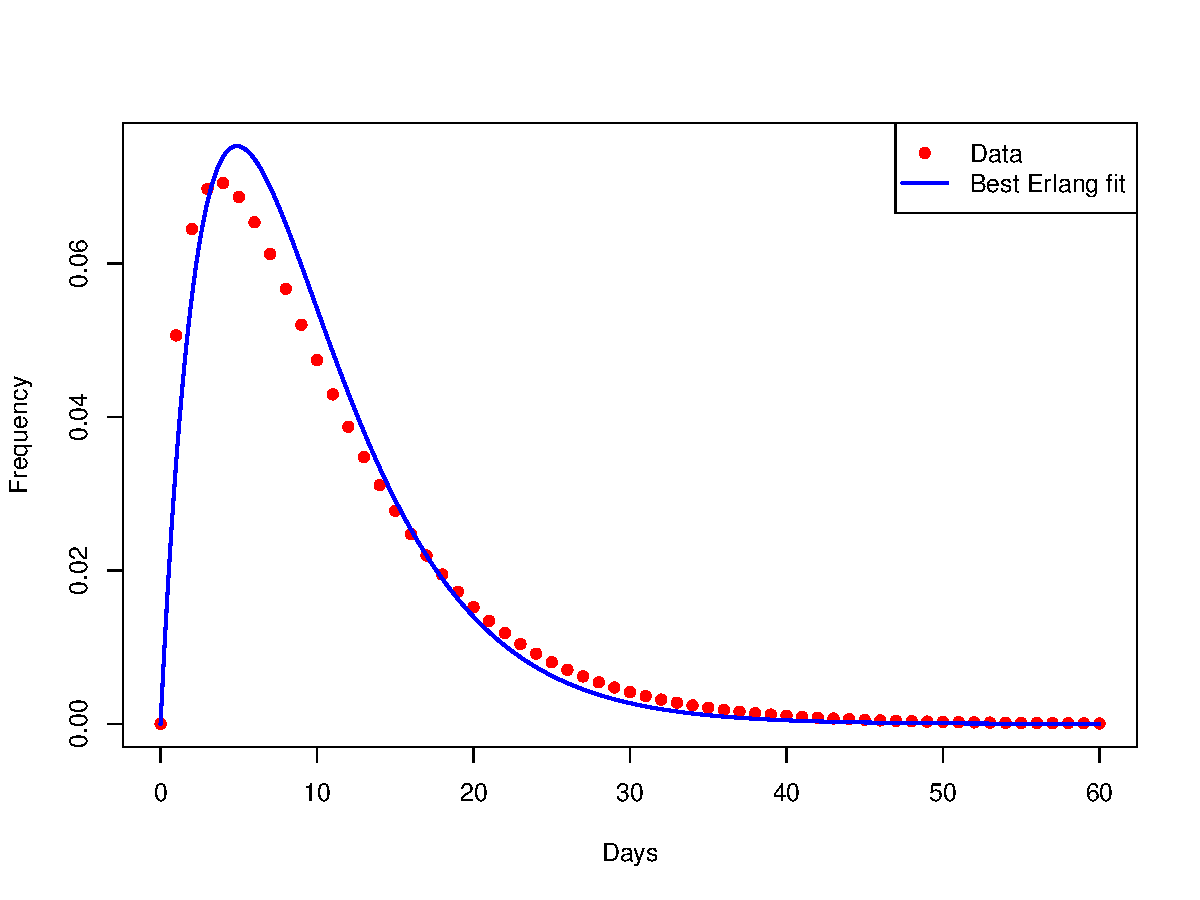
\includegraphics[width=0.75\textwidth]{FIGS/L06-plot_results_optim_Erlang-1.pdf}
\end{center}
\end{frame}



%%%%%%%%%%%%%%%%%%%
%%%%%%%%%%%%%%%%%%%
\subsection{Example -- A COVID-19 model}
\newSubSectionSlide{FIGS-slides-admin/Gemini_Generated_Image_vqpscpvqpscpvqps.jpeg}

\maxFrameImage{FIGS/ArinoPortet-2020.png}
\nocite{ArinoPortet2020}

\begin{frame}
Extends the SLIAR model to take into account non-exponentially distributed stage durations (see lecture 05)
\end{frame}

\begin{frame}{The original model (well, almost the first one)}
\centering
\def\horzskip{*2}
\def\vertskip{*2}
\begin{tikzpicture}[auto, %node distance = 2cm, auto,
	cloud/.style={minimum width={width("N-1")+2pt},
		draw, ellipse,fill=red!20}]
	\node [cloud] (S) at (0,0) {$S$};
	\node [cloud] (L1) at (1\horzskip,0) {$L_1$};
	\node [cloud] (L2) at (2\horzskip,0) {$L_2$};
	\node [cloud,fill=blue!20] (I1) at (3\horzskip,-1\vertskip) {$I_1$};
	\node [cloud] (A1) at (3\horzskip,1\vertskip) {$A_1$};
	\node [cloud,fill=blue!20] (I2) at (4\horzskip,-1\vertskip) {$I_2$};
	\node [cloud] (A2) at (4\horzskip,1\vertskip) {$A_2$};
	\node [cloud,fill=blue!20] (RI) at (5\horzskip,0) {$R_I$};
	\node [cloud] (RA) at (5\horzskip,1\vertskip) {$R_A$};
	\node [cloud,, fill=blue!20] (D) at (5\horzskip,-2\vertskip) {$D$};
	%% Infections
	\path [line, very thick] (S) to node [midway,above] (TextNode) {$\Phi S$} (L1);
	\path [line, very thick] (L1) to node [midway,above] (TextNode) {$\varepsilon L_1$} (L2);
	\path [line, very thick] (L2) to node [midway,below,sloped] (TextNode) {$(1-\pi)\varepsilon L_2$} (I1);
	\path [line, very thick] (L2) to node [midway,below,sloped] (TextNode) {$\pi\varepsilon L_2$} (A1);
	\path [line, very thick] (I1) to node [midway, above] (TextNode) {$\gamma I_1$} (I2);
	\path [line, very thick] (A1) to node [midway, above] (TextNode) {$\gamma A_1$} (A2);
	\path [line, very thick] (I2) to node [midway,above,sloped] (TextNode) {$(1-\delta)\gamma I_2$} (RI);
	\path [line, very thick] (A2) to node [midway, above] (TextNode) {$\gamma A_2$} (RA);
	\path [line, very thick] (I2) to node [midway,below,sloped] (TextNode) {$\delta\gamma I_2$} (D);
\end{tikzpicture}
\end{frame}


\begin{frame}{Reinterpreting terms}
Here $D$ stands for \emph{detected}, $U$ is \emph{undetected}
\vfill
\centering
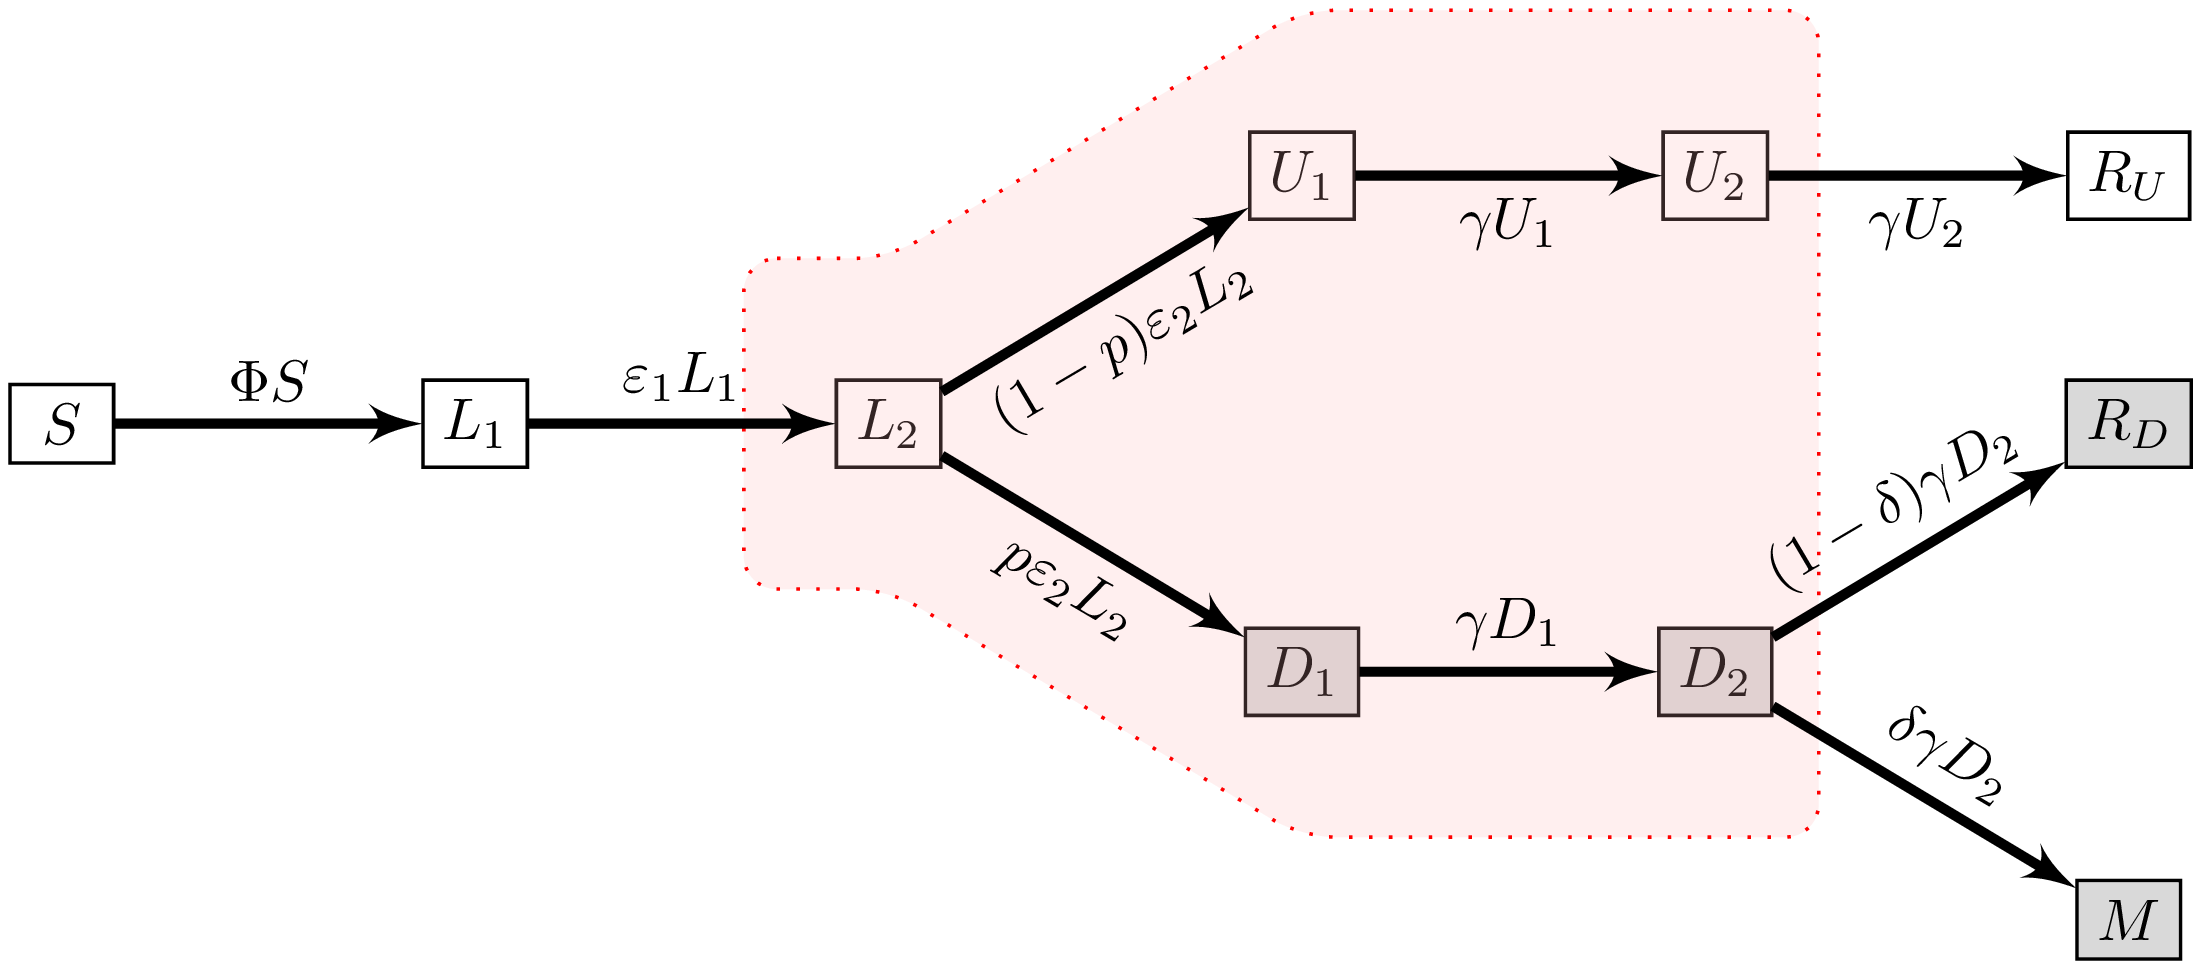
\includegraphics[width=\textwidth]{FIGS/figure_SLDURM_base_model_with_different_epsilon_and_infectious_compartments}
\end{frame}

\begin{frame}{Working out when the first COVID-19 case occurred}
\bbullet Details of emergence and precise timeline before amplification started unknown
\vfill
\bbullet Amplification in Wuhan
\begin{itemize}
\item Cluster of pneumonia cases mostly related to the Huanan Seafood Market
\item 27 December 2019: first report to local government
\item 31 December 2019: publication
\item 8 January 2020: identification of SARS-CoV-2 as causative agent
\item $\sim$ 23 January 2020: lockdown Wuhan and Hubei province + face mask mandates
\end{itemize}
\vfill
\bbullet By 2020-01-29, virus in all provinces of mainland CHN
\end{frame}


\begin{frame}{Evidence of earlier spread}
\bbullet Report to Wuhan authorities on 27 December 2019
\vfill
\bbullet First export detections in Thailand and Japan on 13 and 16 January 2020 (with actual importations on 8 and 6 January)
\vfill
$\implies$ amplification must have been occuring for a while longer
\vfill
\bbullet France: sample taken from 42-year-old male (last foreign travel to Algeria in August 2019) who presented to ICU on 27 December 2019
\vfill
\bbullet Retrospective studies in United Kingdom and Italy also showed undetected COVID-19 cases in prepandemic period
\end{frame}

\begin{frame}{Untangling the first case issue}
\bbullet Robert, Rossman \& Jaric. Dating first cases of COVID-19. \emph{PLoS Pathogens} (2021)

Find likely timing of first case of COVID-19 in China as November 17 (95\% CI October 4)
\vfill
\bbullet Pekar, Worobey, Moshiri, Scheffler \& Wertheim. Timing the SARS-CoV-2 index case in Hubei province. \emph{Science} (2021)

Period between mid-October and mid-November 2019 is plausible interval when the first case of SARS-CoV-2 emerged in Hubei province
\vfill
Important when trying to understand global spread, so let me illustrate with the model I used, taking into account model evolution since
\end{frame}

\begin{frame}{Back-calculating the start of spread (example of China)}
Cumulative confirmed case counts in China as reported to WHO was $c=547$ cases on $t_c=\textrm{2020-01-22}$
\vfill
Let $u$ be a point in parameter space. Solve ODE numerically over $[0,t]$, with $S(0)$ the population of China, $L_1(0)=1$ and other state variables 0. This gives a solution $x(t,t_0=0,u)$
\vfill
Extracting $L_2(t,t_0=0,u)$ from this solution, obtain cumulative number of new detections as
\[
C(t) = \int_{t_0=0}^{t} p\varepsilon_2 L_2(s,t_0,u)\ ds
\]
\vfill
Let $t^\star$ be s.t. $C(t^\star)=547$; then $t_i=\textrm{2020-01-22}-t^\star$
\end{frame}

\begin{frame}
\centering
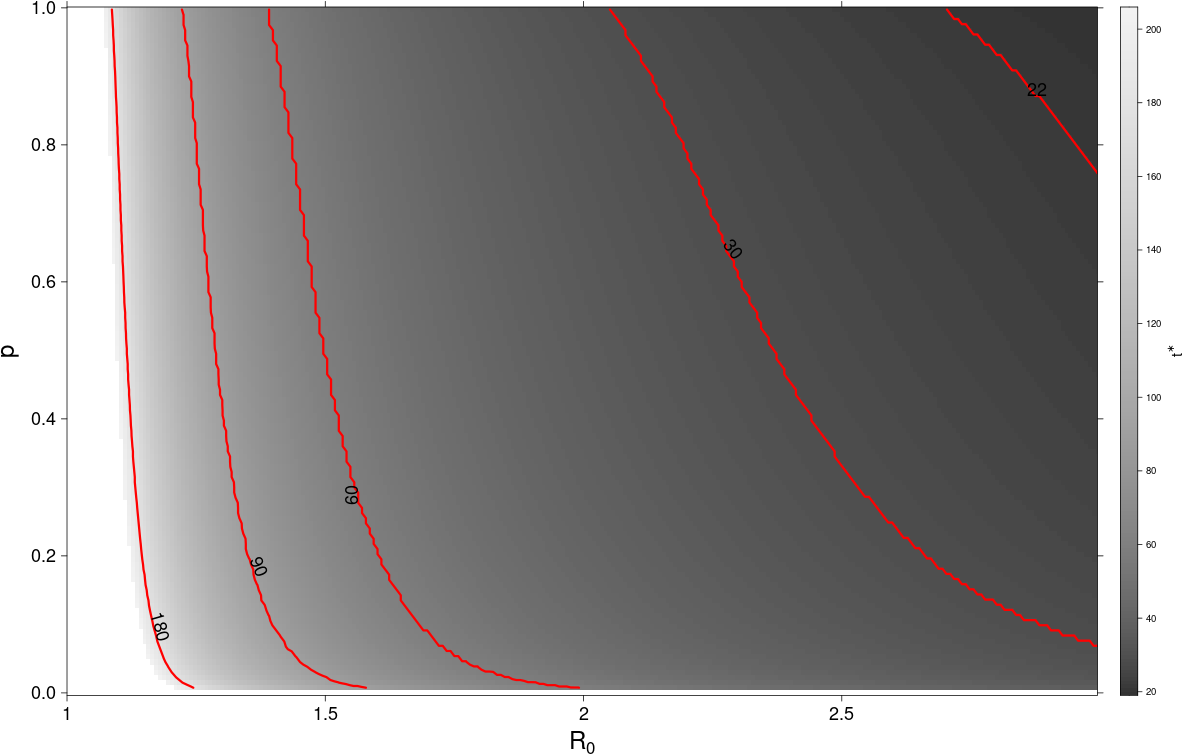
\includegraphics[width=\textwidth]{FIGS/start_time_vs_R0_and_p.png}
\end{frame}



%%%%%%%%%%%%%%%%%%%
%%%%%%%%%%%%%%%%%%%
%%%%%%%%%%%%%%%%%%%
%%%%%%%%%%%%%%%%%%%
\section{Sojourn times in an SIS disease transmission model} 
% The section page
\newSectionSlide{FIGS-slides-admin/Gemini_Generated_Image_5yvymh5yvymh5yvy.jpeg}

\begin{frame}\frametitle{An SIS model}
\framesubtitle{Hypotheses}
\begin{itemize}
\item Individuals typically recover from the disease
\vfill
\item The disease does not confer immunity
\vfill
\item There is no birth or death (from the disease or natural) \newline\imply\;
Constant total population $N\equiv N(t)=S(t)+I(t)$
\vfill
\item Infection is of \defword{standard incidence} type
\end{itemize}
\end{frame}


\begin{frame}\frametitle{Recovery}
\begin{itemize}
\item Traditional models suppose that recovery occurs with rate constant
$\gamma$
\vfill
\item Here, of the individuals that become
infective at time $t_0$, a fraction $\S(t-t_0)$ remain infective at
time $t\geq t_0$
\vfill
\item \imply\;
For $t\geq 0$, $\S(t)$ is a survival function. As such, it verifies
$\S(0)=1$ and $\S$ is nonnegative and nonincreasing
\end{itemize}
\end{frame}


\begin{frame}\frametitle{Model for infectious individuals}
Since $N$ is constant, $S(t)=N-I(t)$ and we need only
consider the following equation (where $S$ is used for clarity)
\begin{equation}
I(t) = I_0(t)+ \int_0^t\beta\frac{S(u)I(u)}{N} \S(t-u) du
\label{eq:SIS_I} 
\end{equation}
\vfill
\begin{itemize}
\item $I_0(t)$ number of individuals who were infective at time
$t=0$ and still are at time $t$
\begin{itemize}
\item $I_0(t)$ is nonnegative, nonincreasing, and
such that $\lim_{t\to\infty}I_0(t)=0$
\end{itemize}
\item $\S(t-u)$ proportion of individuals who became infective at time $u$ and who still are at time $t$
\end{itemize}
\end{frame}


\begin{frame}\frametitle{Expression under the integral}
Integral equation for the number of infective individuals: 
\begin{equation}
I(t) = I_0(t)+ \int_0^t\beta\frac{(N-I(u))I(u)}{N} \S(t-u) du
\tag{\ref{eq:SIS_I}} 
\end{equation}
The term
\[
\beta\frac{(N-I(u))I(u)}{N} \S(t-u)
\]
\begin{itemize}
\item $\beta (N-I(u))I(u)/N$ is the rate at which new infectives are created, at time $u$
\item multiplying by $\S(t-u)$ gives the proportion of those who became
infectives at time $u$ and who still are at time $t$
\end{itemize}
Summing over $[0,t]$ gives the number of infective individuals at time $t$
\end{frame}


\begin{frame}\frametitle{Case of an exponentially distributed time to recovery}
Suppose $\S(t)$ such that sojourn time in the infective
state has exponential distribution with mean $1/\gamma$,
\textit{i.e.}, $\S(t)=e^{-\gamma t}$
\vfill
Initial condition function $I_0(t)$ takes the form
\[
I_0(t)=I_0(0)e^{-\gamma t}
\]
with $I_0(0)$ the number of infective individuals at time $t=0$. Obtained by considering the cohort of initially infectious individuals, giving a
model such as \eqref{eq:N_general}
\vfill
Equation (\ref{eq:SIS_I}) becomes
\begin{equation}\label{eq:I_ODE}
I(t)=I_0(0)e^{-\gamma t}+\int_0^t \beta\frac{(N-I(u))I(u)}{N} e^{-\gamma
(t-u)}du
\end{equation}
\end{frame}

\begin{frame}
Taking the time derivative of \eqref{eq:I_ODE} yields
\begin{align*}
I'(t) &= -\gamma I_0(0)e^{-\gamma t}-\gamma\int_0^t
\beta\frac{(N-I(u))I(u)}{N}e^{-\gamma(t-u)}du \\
&\quad +\beta \frac{(N-I(t))I(t)}{N} \\
&= -\gamma\left(I_0(0)e^{-\gamma t}+
\int_0^t \beta\frac{(N-I(u))I(u)}{N}e^{-\gamma(t-u)}du\right) \\
&\quad +\beta \frac{(N-I(t))I(t)}{N} \\
&= \beta \frac{(N-I(t))I(t)}{N}-\gamma I(t)
\end{align*}
\vfill
This is the classical logistic type ordinary differential equation (ODE) for $I$ in an SIS model without vital dynamics (no birth or death)
\end{frame}



\begin{frame}\frametitle{Case of a step function survival function}
Consider case where the time spent infected has survival function 
\[
\S(t)=\begin{cases}
1, & 0\leq t\leq\omega,\\
0, & t>\omega.
\end{cases}
\]
i.e., the sojourn time in the infective state is a constant
$\omega>0$
\vfill
In this case (\ref{eq:SIS_I}) becomes
\begin{equation}\label{eq:I_DDE}
I(t)=I_0(t)+\int_{t-\omega}^t \beta\frac{(N-I(u))I(u)}{N} du.
\end{equation}
Here, it is more difficult to obtain an expression for $I_0(t)$. It is however assumed that $I_0(t)$ vanishes for $t>\omega$
\end{frame}

\begin{frame}
When differentiated, \eqref{eq:I_DDE} gives, for $t\geq\omega$,
\[
I'(t)=I_0'(t)+\beta\frac{(N-I(t))I(t)}{N}
-\beta\frac{\left(N-I(t-\omega)\right)I(t-\omega)}{N}.
\]
Since $I_0(t)$ vanishes for $t>\omega$, this gives the delay
differential equation (DDE)
\[
I'(t)=\beta\frac{(N-I(t))I(t)}{N}
-\beta\frac{(N-I(t-\omega))I(t-\omega)}{N}.
\]
\end{frame}









%%%%%%%%%%%%%%%%%%%
%%%%%%%%%%%%%%%%%%%
%%%%%%%%%%%%%%%%%%%
%%%%%%%%%%%%%%%%%%%



%%%%%%%%%%%%%%%%%%%
%%%%%%%%%%%%%%%%%%%
%%%%%%%%%%%%%%%%%%%
%%%%%%%%%%%%%%%%%%%
\begin{frame}[allowframebreaks]{Bibliography}
\bibliographystyle{apalike}
\bibliography{local-bibliography}
\end{frame}




\end{document}
